This chapter compares a suite of weak lensing statistics derived from two sets of simulations: BIGBOX and TILED. Our goal is to quantify differences in mean values, covariance, and correlation matrices to assess how super-sample covariance and other systematic effects influence these measurements. We will also examine how shape noise, smoothing scales, and box replication artifacts affect the results.
Unless otherwise specified, the main results presented are derived from noiseless simulations with a smoothing scale of $2$ arcmins.

\section{Comparison of Mean and Variance for Statistical Measures}
We analyze and compare the mean values ($\mu$) and variances ($\sigma^2$) of statistical measures derived from the BIGBOX and TILED simulations. Figures~\ref{fig:ell_main} and~\ref{fig:nu_main} illustrate these comparisons for the angular power spectrum, bispectrum, and other higher-order statistics, providing insight into the differences introduced by simulation methodologies and super-sample covariance effects.

The mean values, represented by the ratio $R_{\mu}$, show remarkable consistency between the two simulation sets. For most statistics, the deviations in $R_{\mu}$ remain below $1\%$, highlighting the robustness of both simulation pipelines in capturing the underlying statistical distributions. However, systematic deviations arise at low $\nu$ values for peak counts, minima, and Minkowski Functionals. These deviations likely reflect the inability of the TILED simulations to adequately resolve low-density regions.

In contrast, the variance ratios $R_{\sigma^2}$ reveal more pronounced differences, emphasizing the role of super-sample covariance. The variance ratio for the angular power spectrum exhibits significant enhancement in the BIGBOX simulations at high $\ell$. This behavior aligns with the expected amplification of variance due to the inclusion of larger-scale modes in the BIGBOX setup, which are absent in the TILED simulations. Furthermore, the discrepancy between variance ratios becomes increasingly pronounced with higher source redshifts, consistent with the progressive loss of large-scale modes in the TILED simulations. For $\nu$-binned statistics, the BIGBOX simulations consistently yield higher variances across nearly all $\nu$ bins. This trend is amplified at greater source redshifts, with the ratios of variances demonstrating a systematic increase. These findings underscore the influence of super-sample covariance on higher-order statistics. 

\begin{figure}[ht]
    \centering
    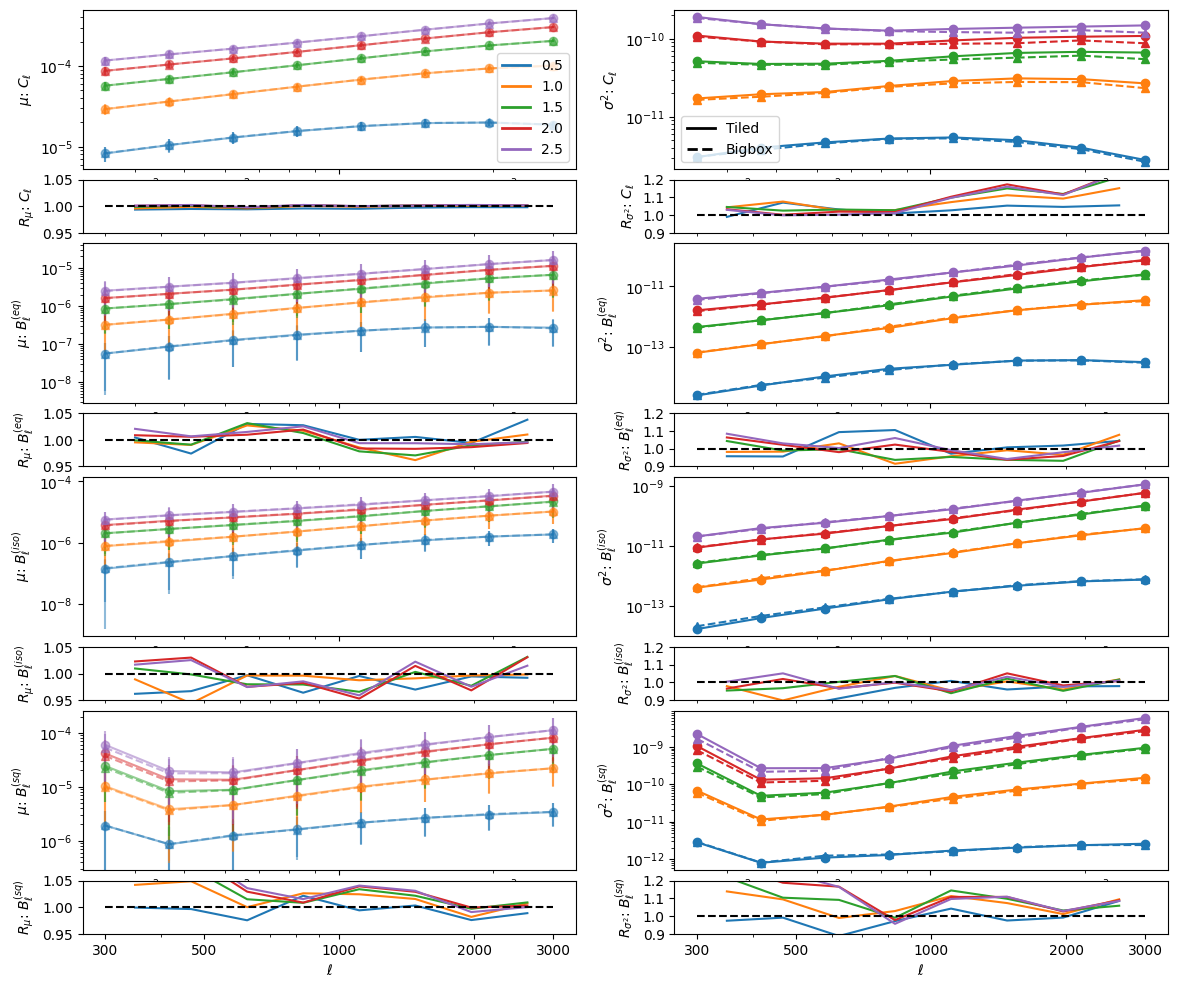
\includegraphics[width=\textwidth]{figures/results/ell_main.png}
    \caption[Comparison of Mean and Variance for $C^{\kappa\kappa}_{\ell}$ and Bispectrum]
    {Comparison of the mean and variance for the angular power spectrum ($C^{\kappa\kappa}_{\ell}$) and the bispectrum across three configurations: equilateral ($B_{\ell}^{(eq)}$), isosceles ($B_{\ell}^{(iso)}$), and squeezed ($B_{\ell}^{(sq)}$). Results are shown for the BIGBOX and TILED simulations at multiple source redshifts ($z_s = 0.5, 1.0, 1.5, 2.0, 2.5$).}
    \label{fig:ell_main}
\end{figure}

\begin{figure}[p]
    \centering
    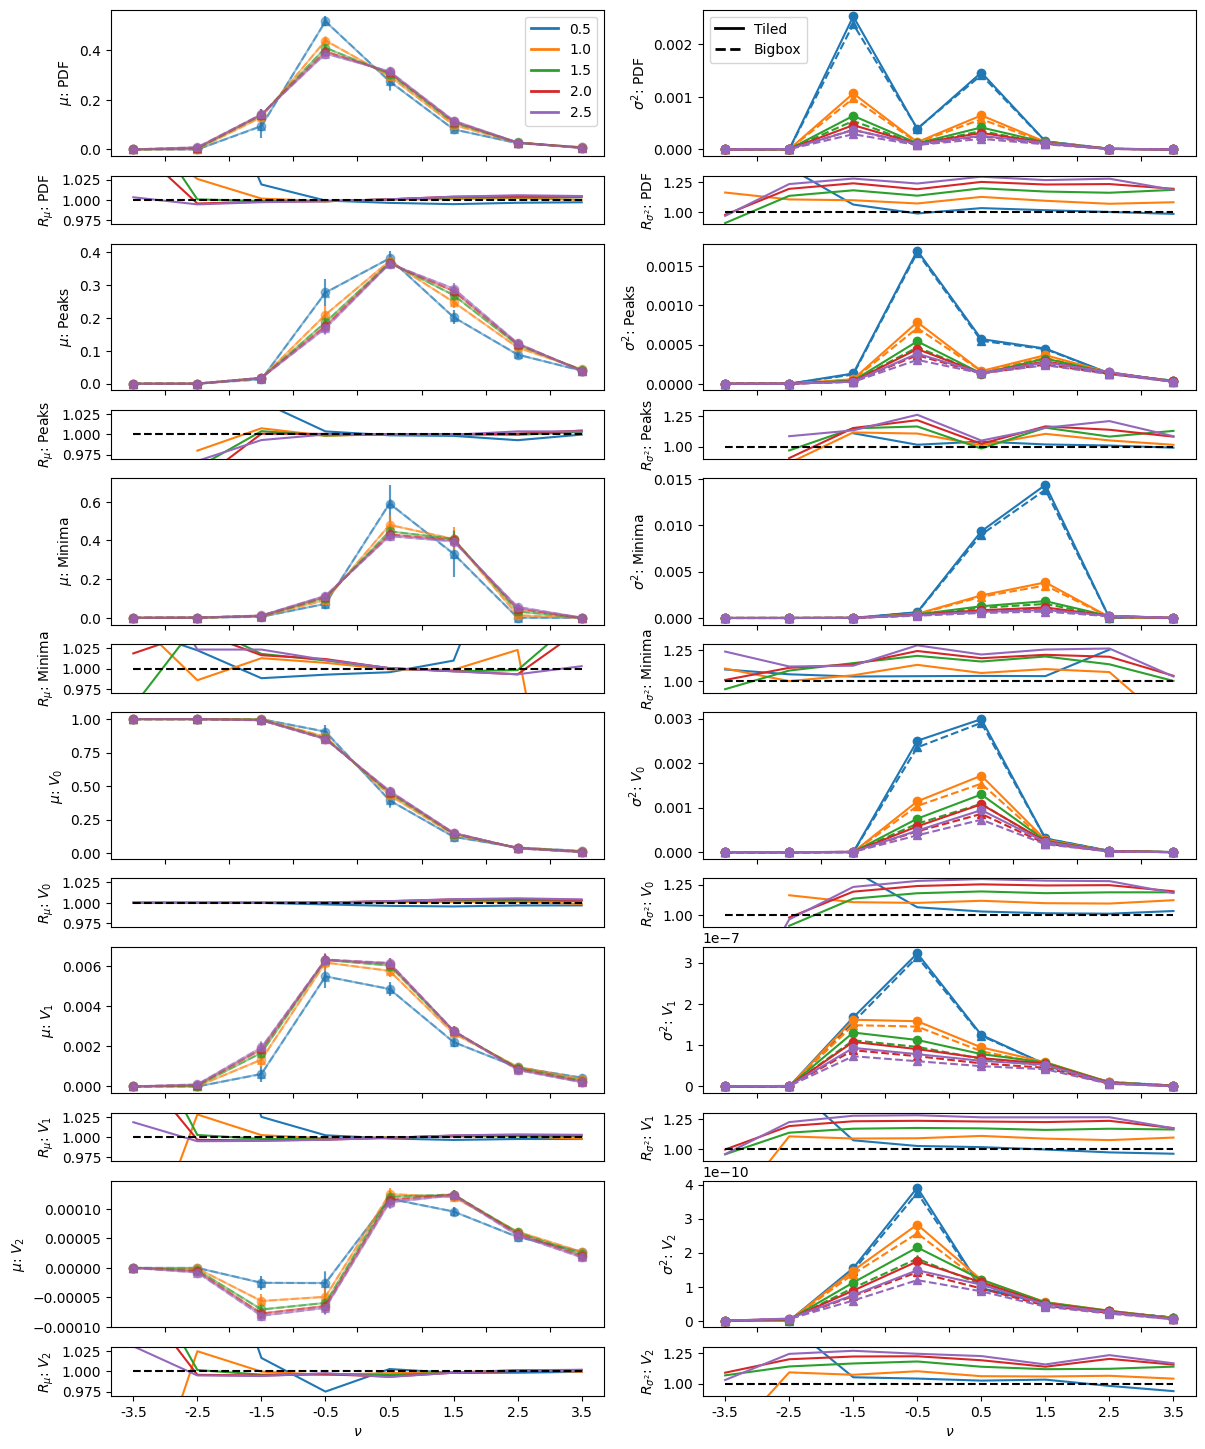
\includegraphics[width=\textwidth]{figures/results/nu_main.png}
    \caption[Comparison of Mean and Variance for Non-Correlation Statistics]
    {Comparison of the mean and variance for non-correlation-based statistics, including the probability density function (PDF), peak and minima counts, and the Minkowski Functionals ($V_0$, $V_1$, $V_2$). Results are derived from the BIGBOX and TILED simulations at multiple source redshifts ($z_s = 0.5, 1.0, 1.5, 2.0, 2.5$), demonstrating the sensitivity of these measures to super-sample covariance.}
    \label{fig:nu_main}
\end{figure}

\clearpage

\section{Analysis of Covariance and Correlation Matrices}
To quantify the super-sample covariance effects on off-diagonal terms, we also compare the covariance and correlation matrices of the statistical measures. 

Figure~\ref{fig:cov_bigbox} shows the covariance matrices for the BIGBOX simulations, while Figure~\ref{fig:cov_tiled} displays the corresponding matrices for the TILED simulations. The general covariance structures are consistent between the two simulation sets, with the BIGBOX simulations exhibiting higher covariance values.Figure~\ref{fig:corr_main} illustrates the correlation matrices for the BIGBOX and TILED simulations. The upper-left triangle of each panel shows the correlation coefficients dericed from the BIGBOX simulations, while the lower-right triangle displays the corresponding values from the TILED simulations. There is no obivious discrepancies in this color scale, indicating that the correlation structures are consistent between the two simulation sets.

Figures~\ref{fig:cov_ratio_main} and~\ref{fig:corr_ratio_main} illustrate the ratios of covariance and correlation matrices between the BIGBOX and TILED simulations, denoted as $R_{\text{Cov}}$ and $R_{\rho}$, respectively. These comparisons provide a quantitative assessment of the influence of super-sample covariance on both diagonal and off-diagonal elements of the covariance structure. The covariance ratios $R_{\text{Cov}}$ generally exceed unity, ranging from $10\%$ to $30\%$ above baseline for most statistical measures. This consistent elevation underscores the significant contribution of super-sample covariance to the overall covariance matrix. Conversely, the correlation ratios $R_{\rho}$ only deviates typically $ < 5\%$. These results suggest that the super-sample effect impacts not only the diagonal terms but also the off-diagonal elements of the covariance matrix, thereby lifting the entire structure. Notable exceptions to these trends occur in the angular power spectrum and peak/minima counts. For the angular power spectrum, larger deviations in the correlation ratios are consistent with super-sample covariance effects. These arise from the strong correlations introduced by shared large-scale modes, particularly between small $\ell$. In contrast, the deviations observed in the peak/minima counts are likely attributable to systematic shifts in peak positions within the TILED simulations, which affect correlations around the peak bins. For a summary of the average ratios of covariance and correlation matrices, see Figure~\ref{fig:avg_main}.

\begin{figure}[ht]
    \begin{minipage}{0.48\textwidth}
        \centering
        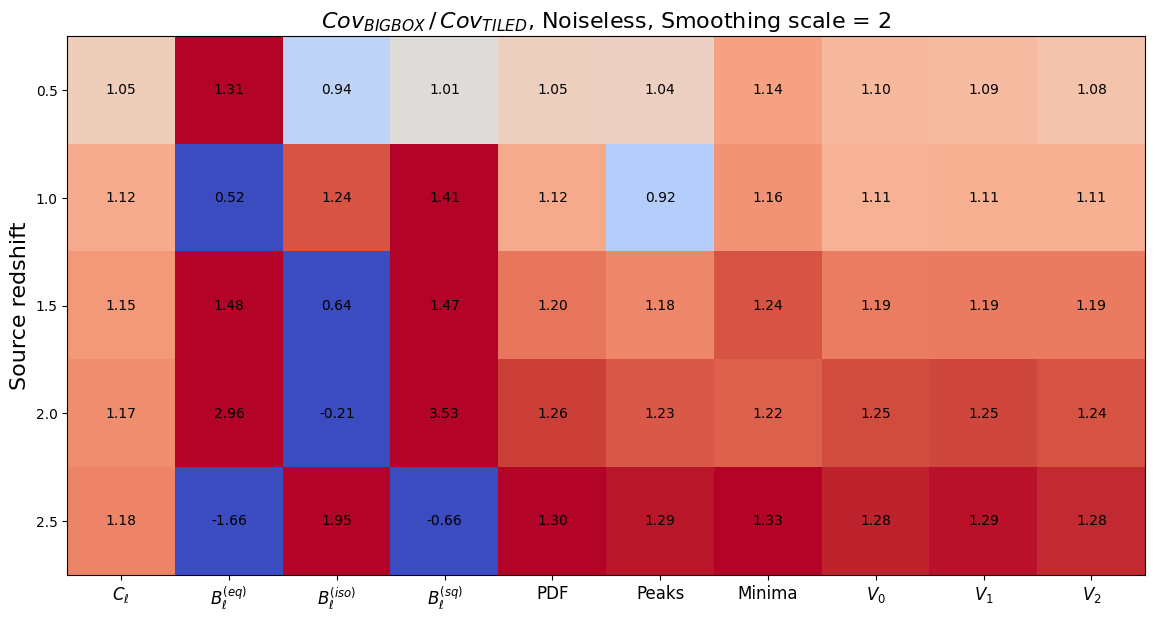
\includegraphics[width=\textwidth]{figures/results/avg_cov_ratio_main.png}
    \end{minipage}
    \begin{minipage}{0.48\textwidth}
        \centering
        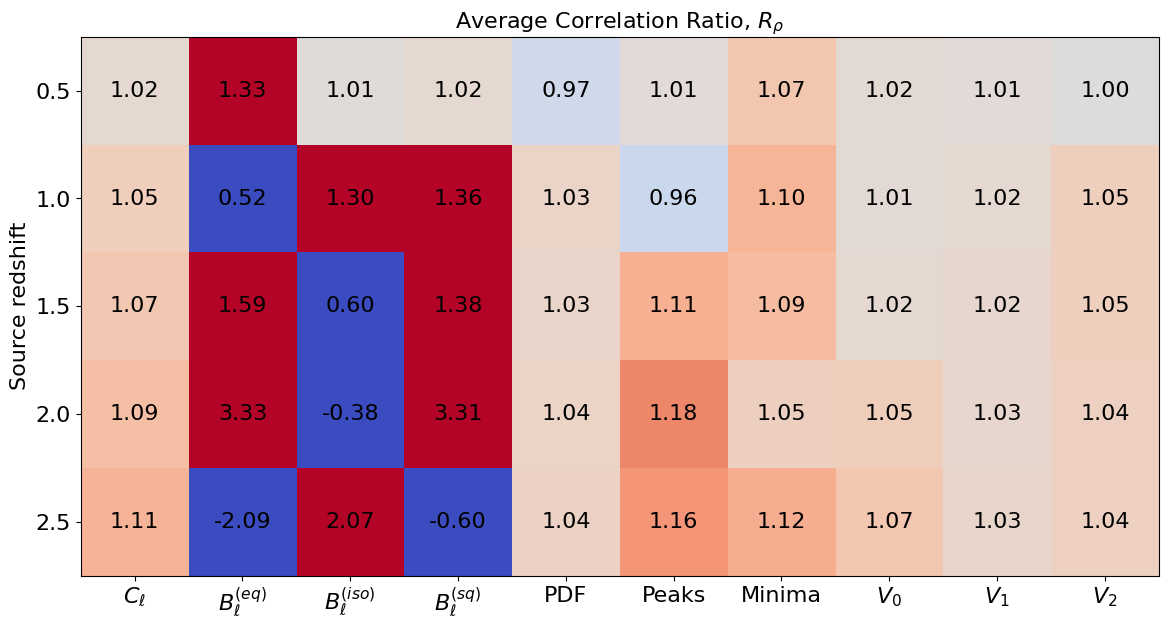
\includegraphics[width=\textwidth]{figures/results/avg_corr_ratio_main.png}
    \end{minipage}
    \caption[Average BIGBOX/TILED Ratios of Covariance and Correlation Matrices]{Average ratios of covariance matrices (left) and correlation matrices (right) between the BIGBOX and TILED simulations for multiple source redshifts. The increasing trend in the covariance ratios indicates the impact of super-sample covariance on the covariance structures.}
    \label{fig:avg_main}
\end{figure}

\begin{figure}[p]
    \centering
    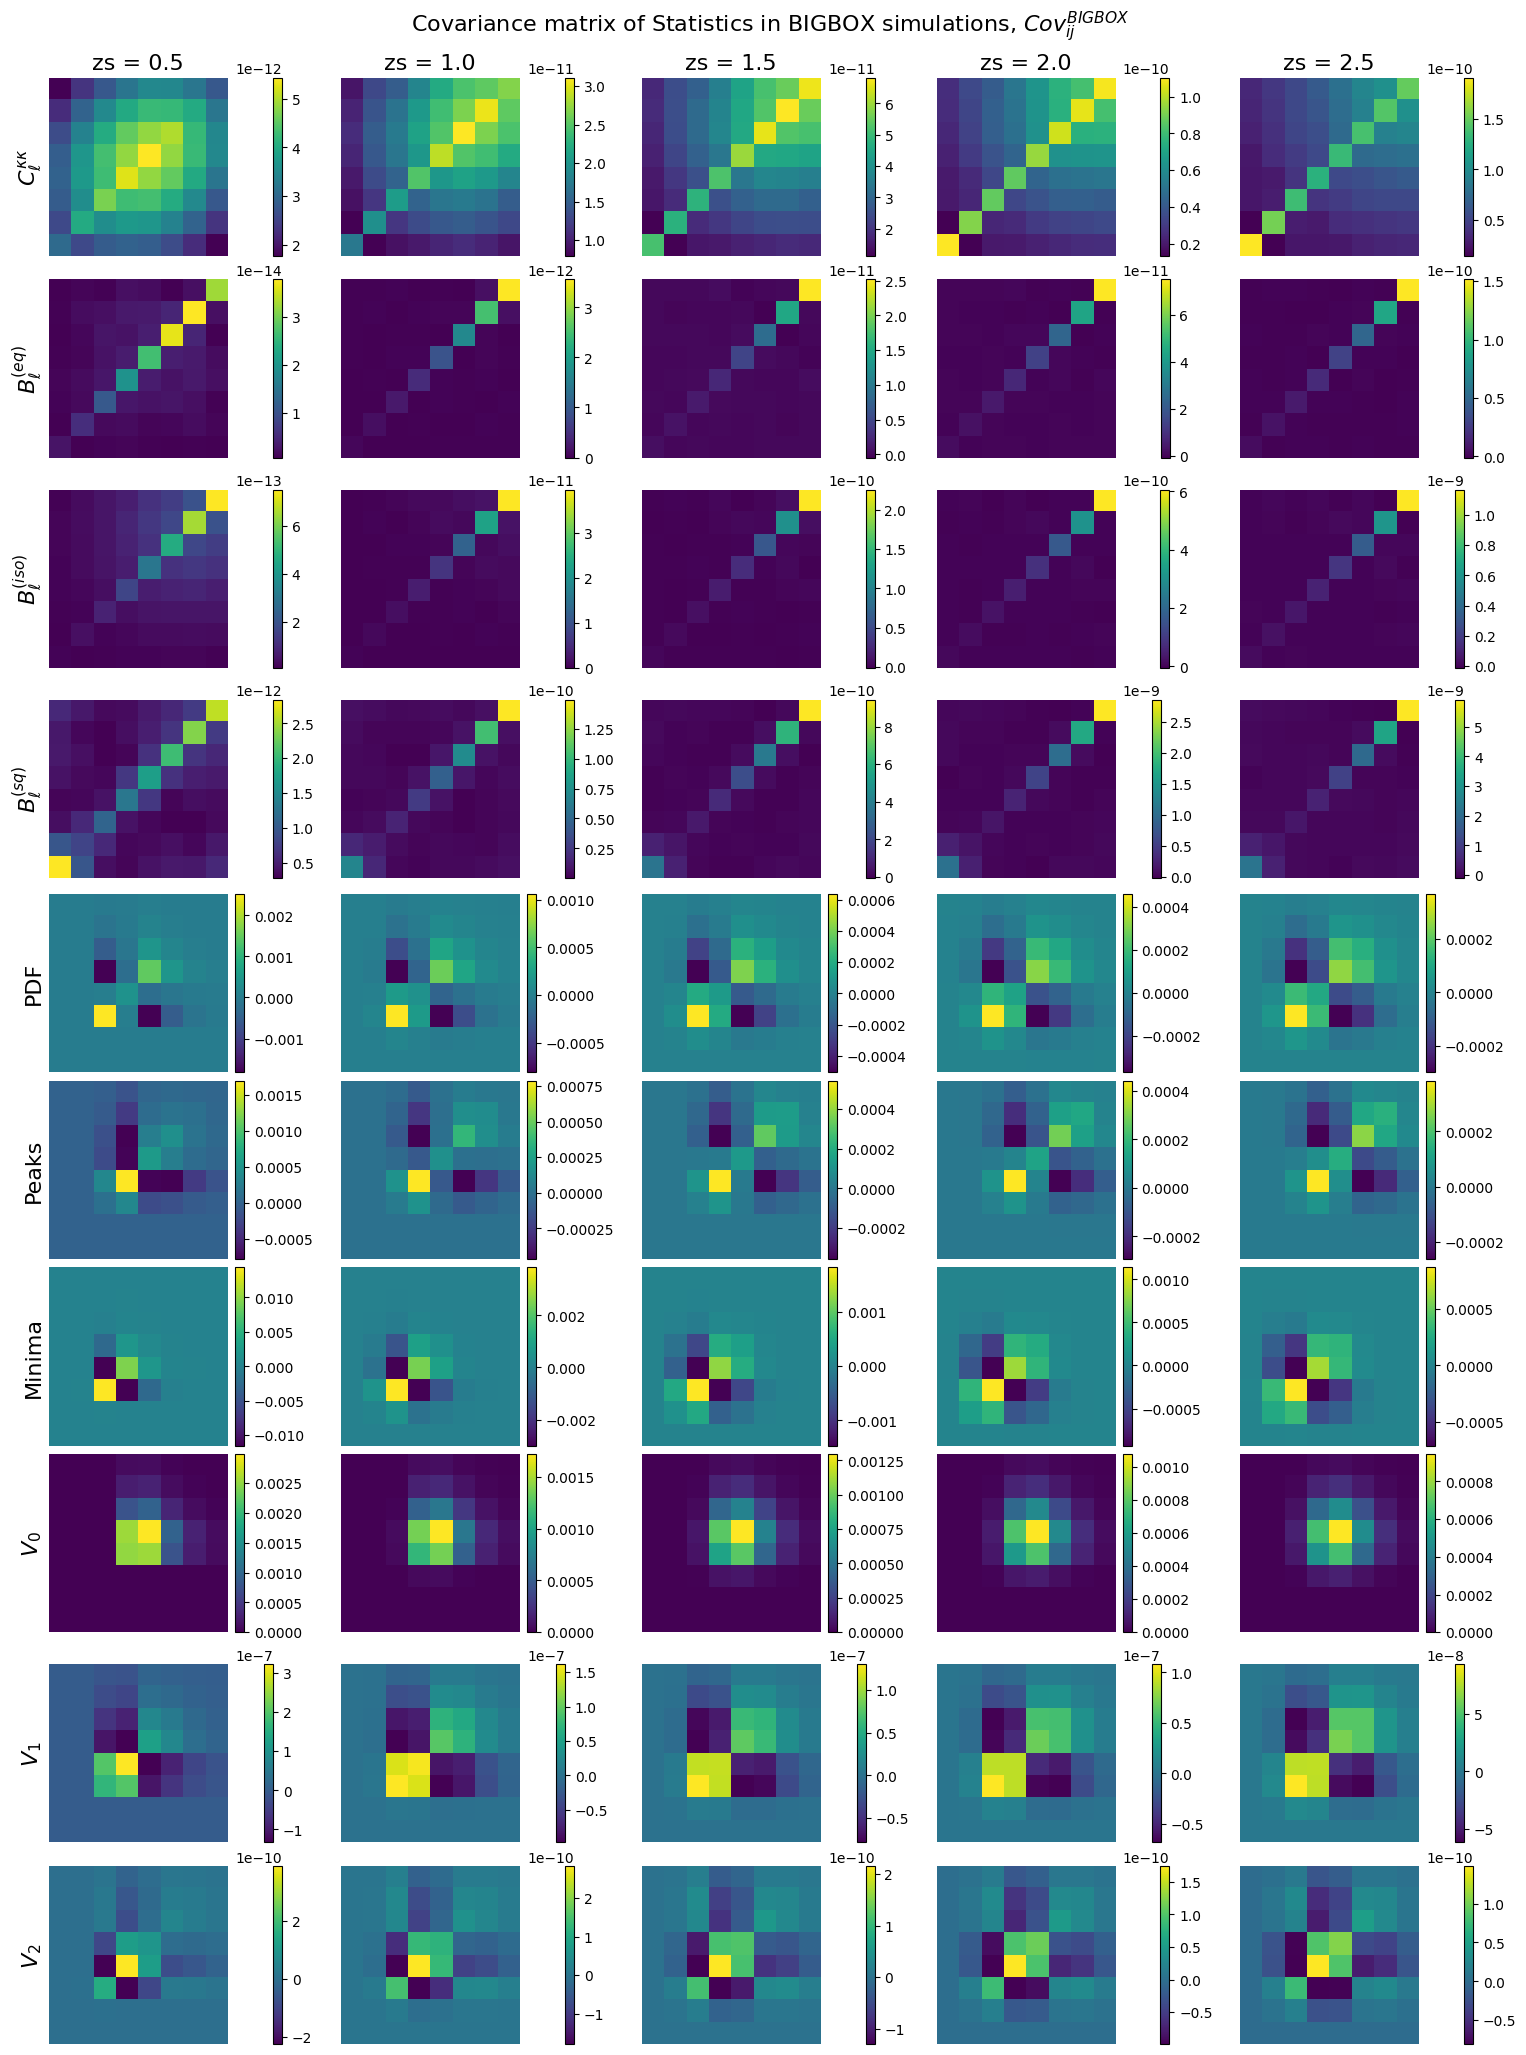
\includegraphics[width=\textwidth]{figures/results/cov_bigbox.png}
    \caption[Covariance Matrices of Statistical Measures in BIGBOX Simulations]{Covariance matrices of statistical measures in the BIGBOX simulations for multiple source redshifts.}
    \label{fig:cov_bigbox}
\end{figure}

\begin{figure}[p]
    \centering
    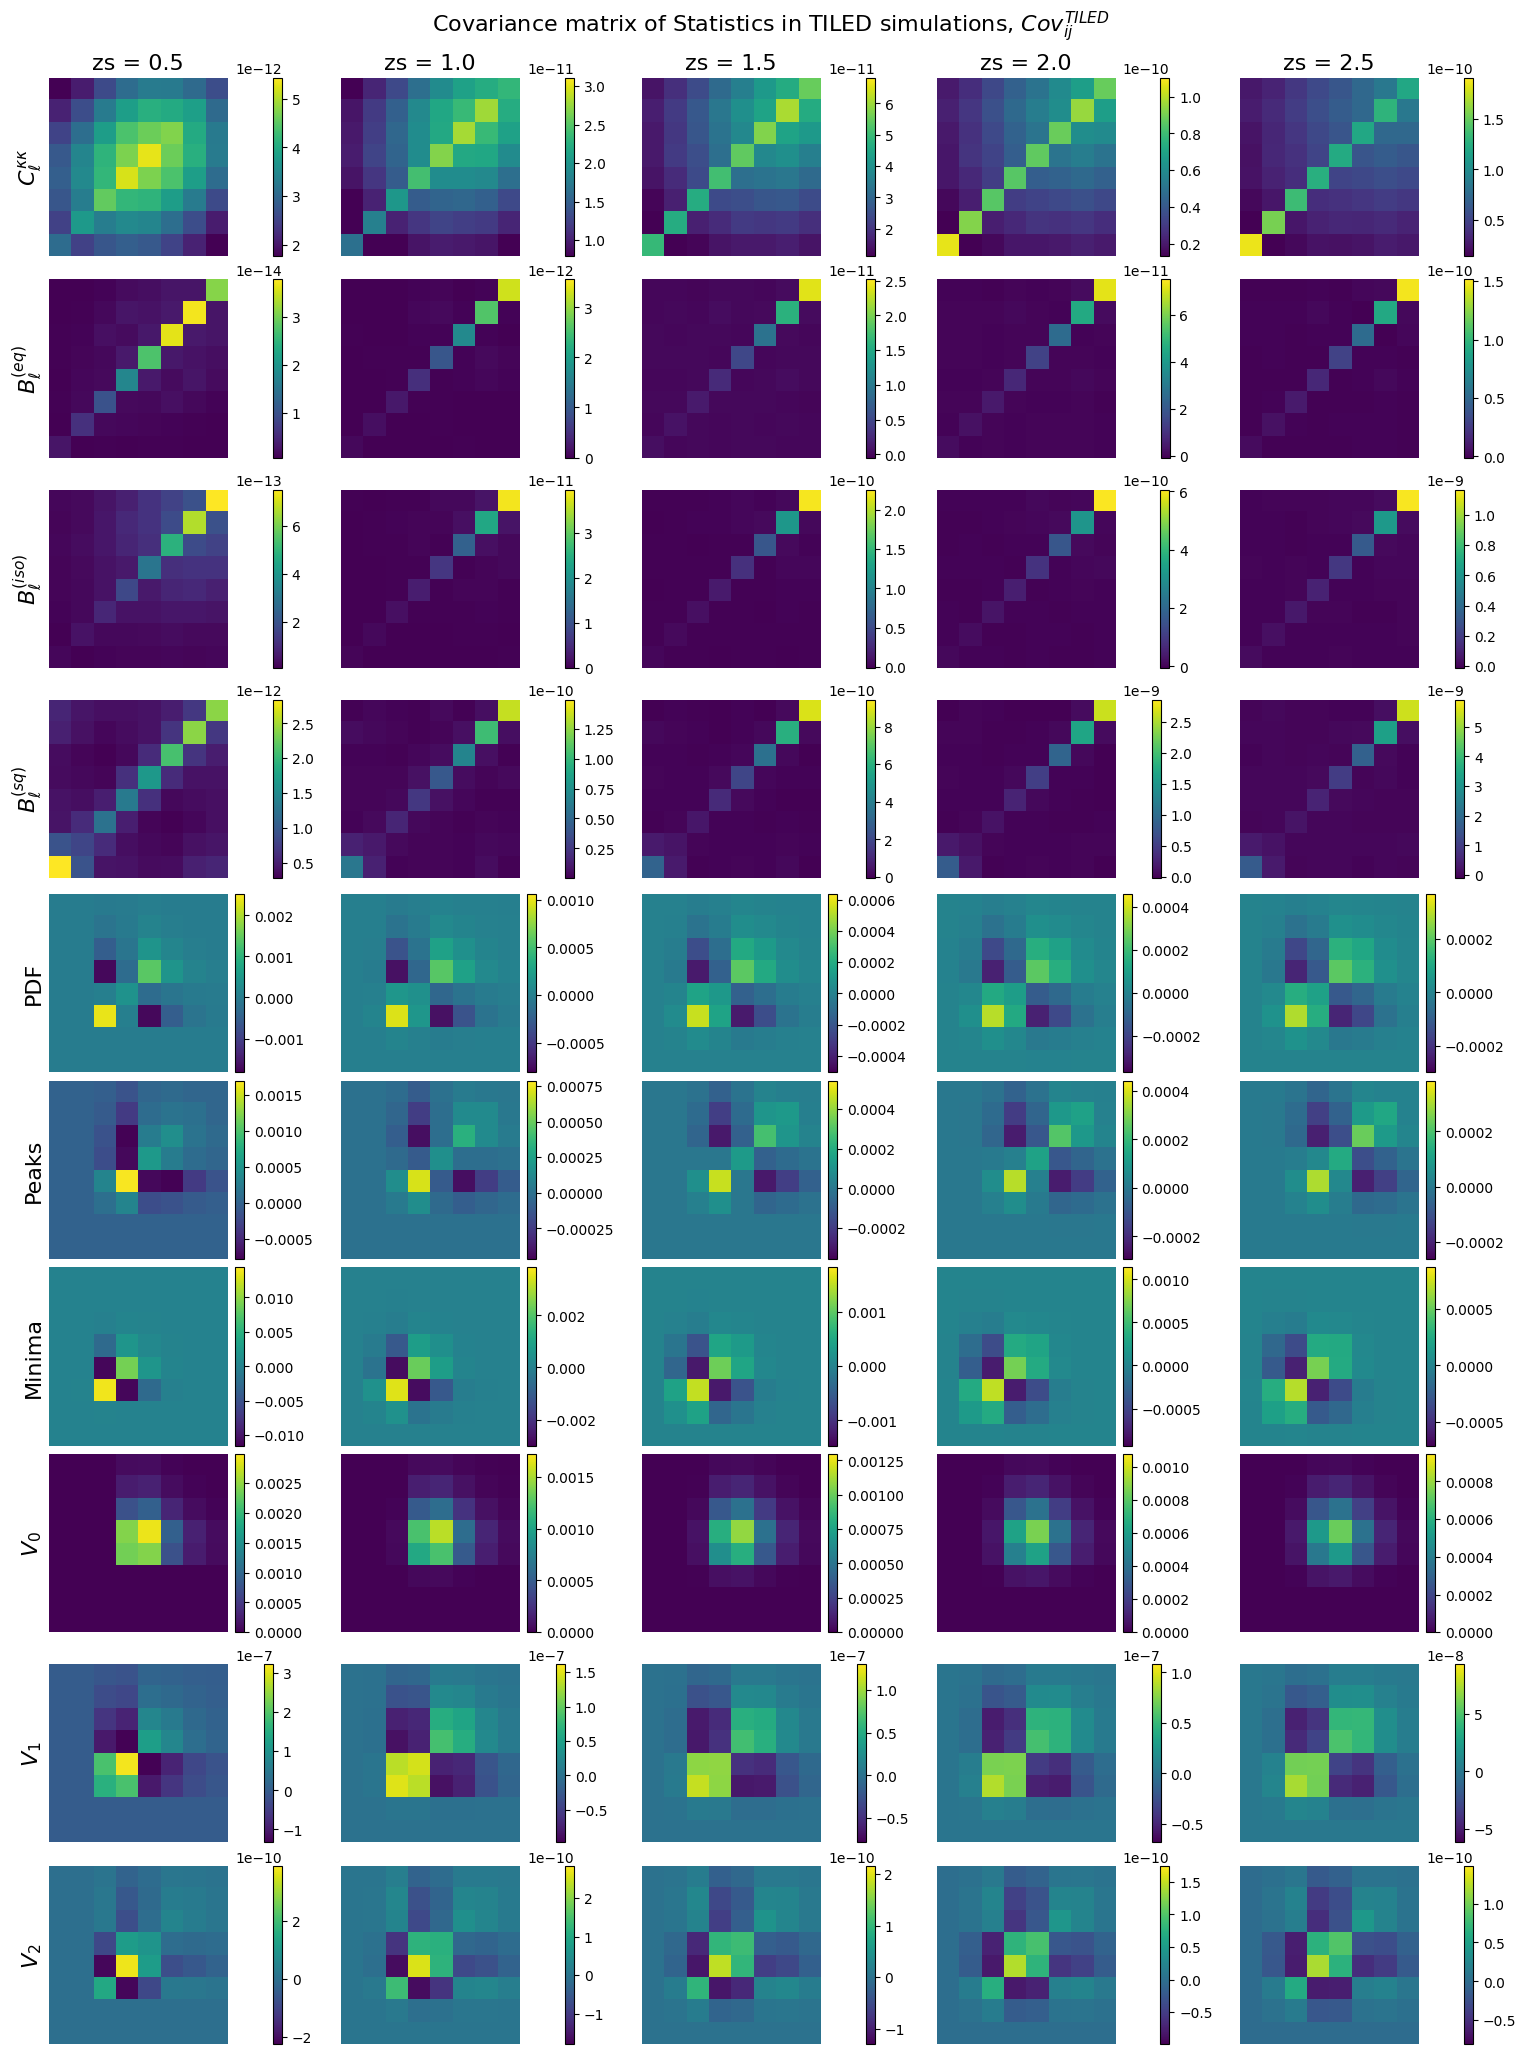
\includegraphics[width=\textwidth]{figures/results/cov_tiled.png}
    \caption[Covariance Matrices of Statistical Measures in TILED Simulations]{Covariance matrices of statistical measures in the TILED simulations for multiple source redshifts. The color scale is consistent with the corresponding panels in Figure~\ref{fig:cov_bigbox}.}
    \label{fig:cov_tiled}
\end{figure}

\begin{figure}[p]
    \centering
    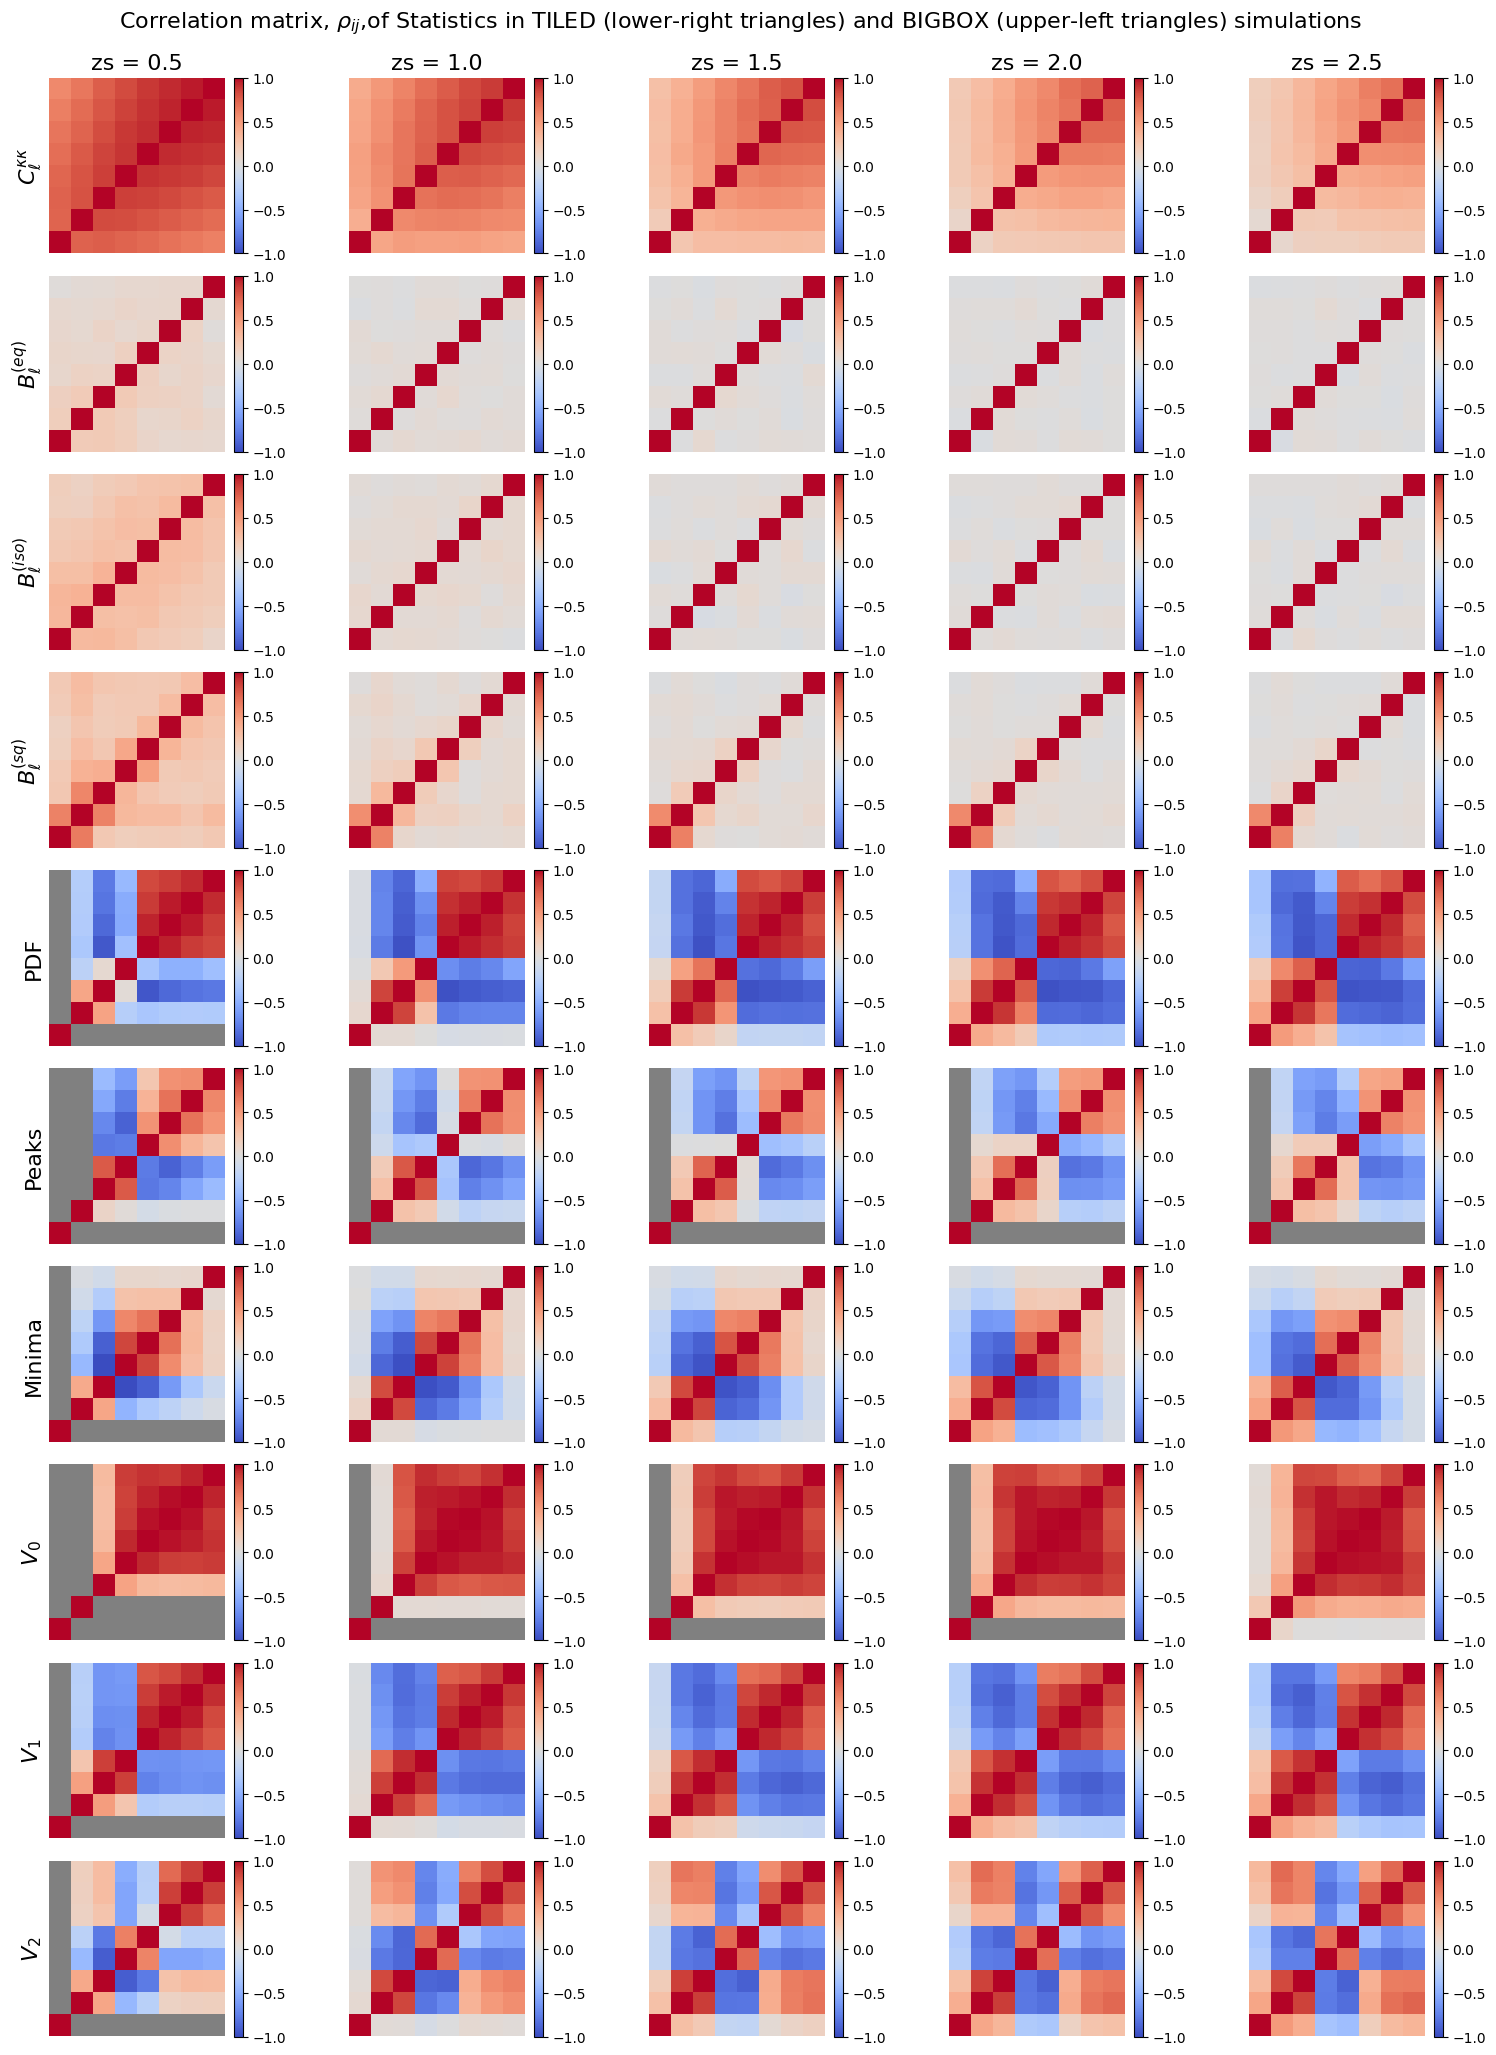
\includegraphics[width=\textwidth]{figures/results/corr_main.png}
    \caption[Correlation Matrices of Statistical Measures in BIGBOX and TILED Simulations]{Correlation matrices of statistical measures in the BIGBOX and TILED simulations for multiple source redshifts. The upper-left triangle shows the correlation coefficients derived from the BIGBOX simulations, while the lower-right triangle displays the corresponding values from the TILED simulations.}
    \label{fig:corr_main}
\end{figure}

\begin{figure}[p]
    \centering
    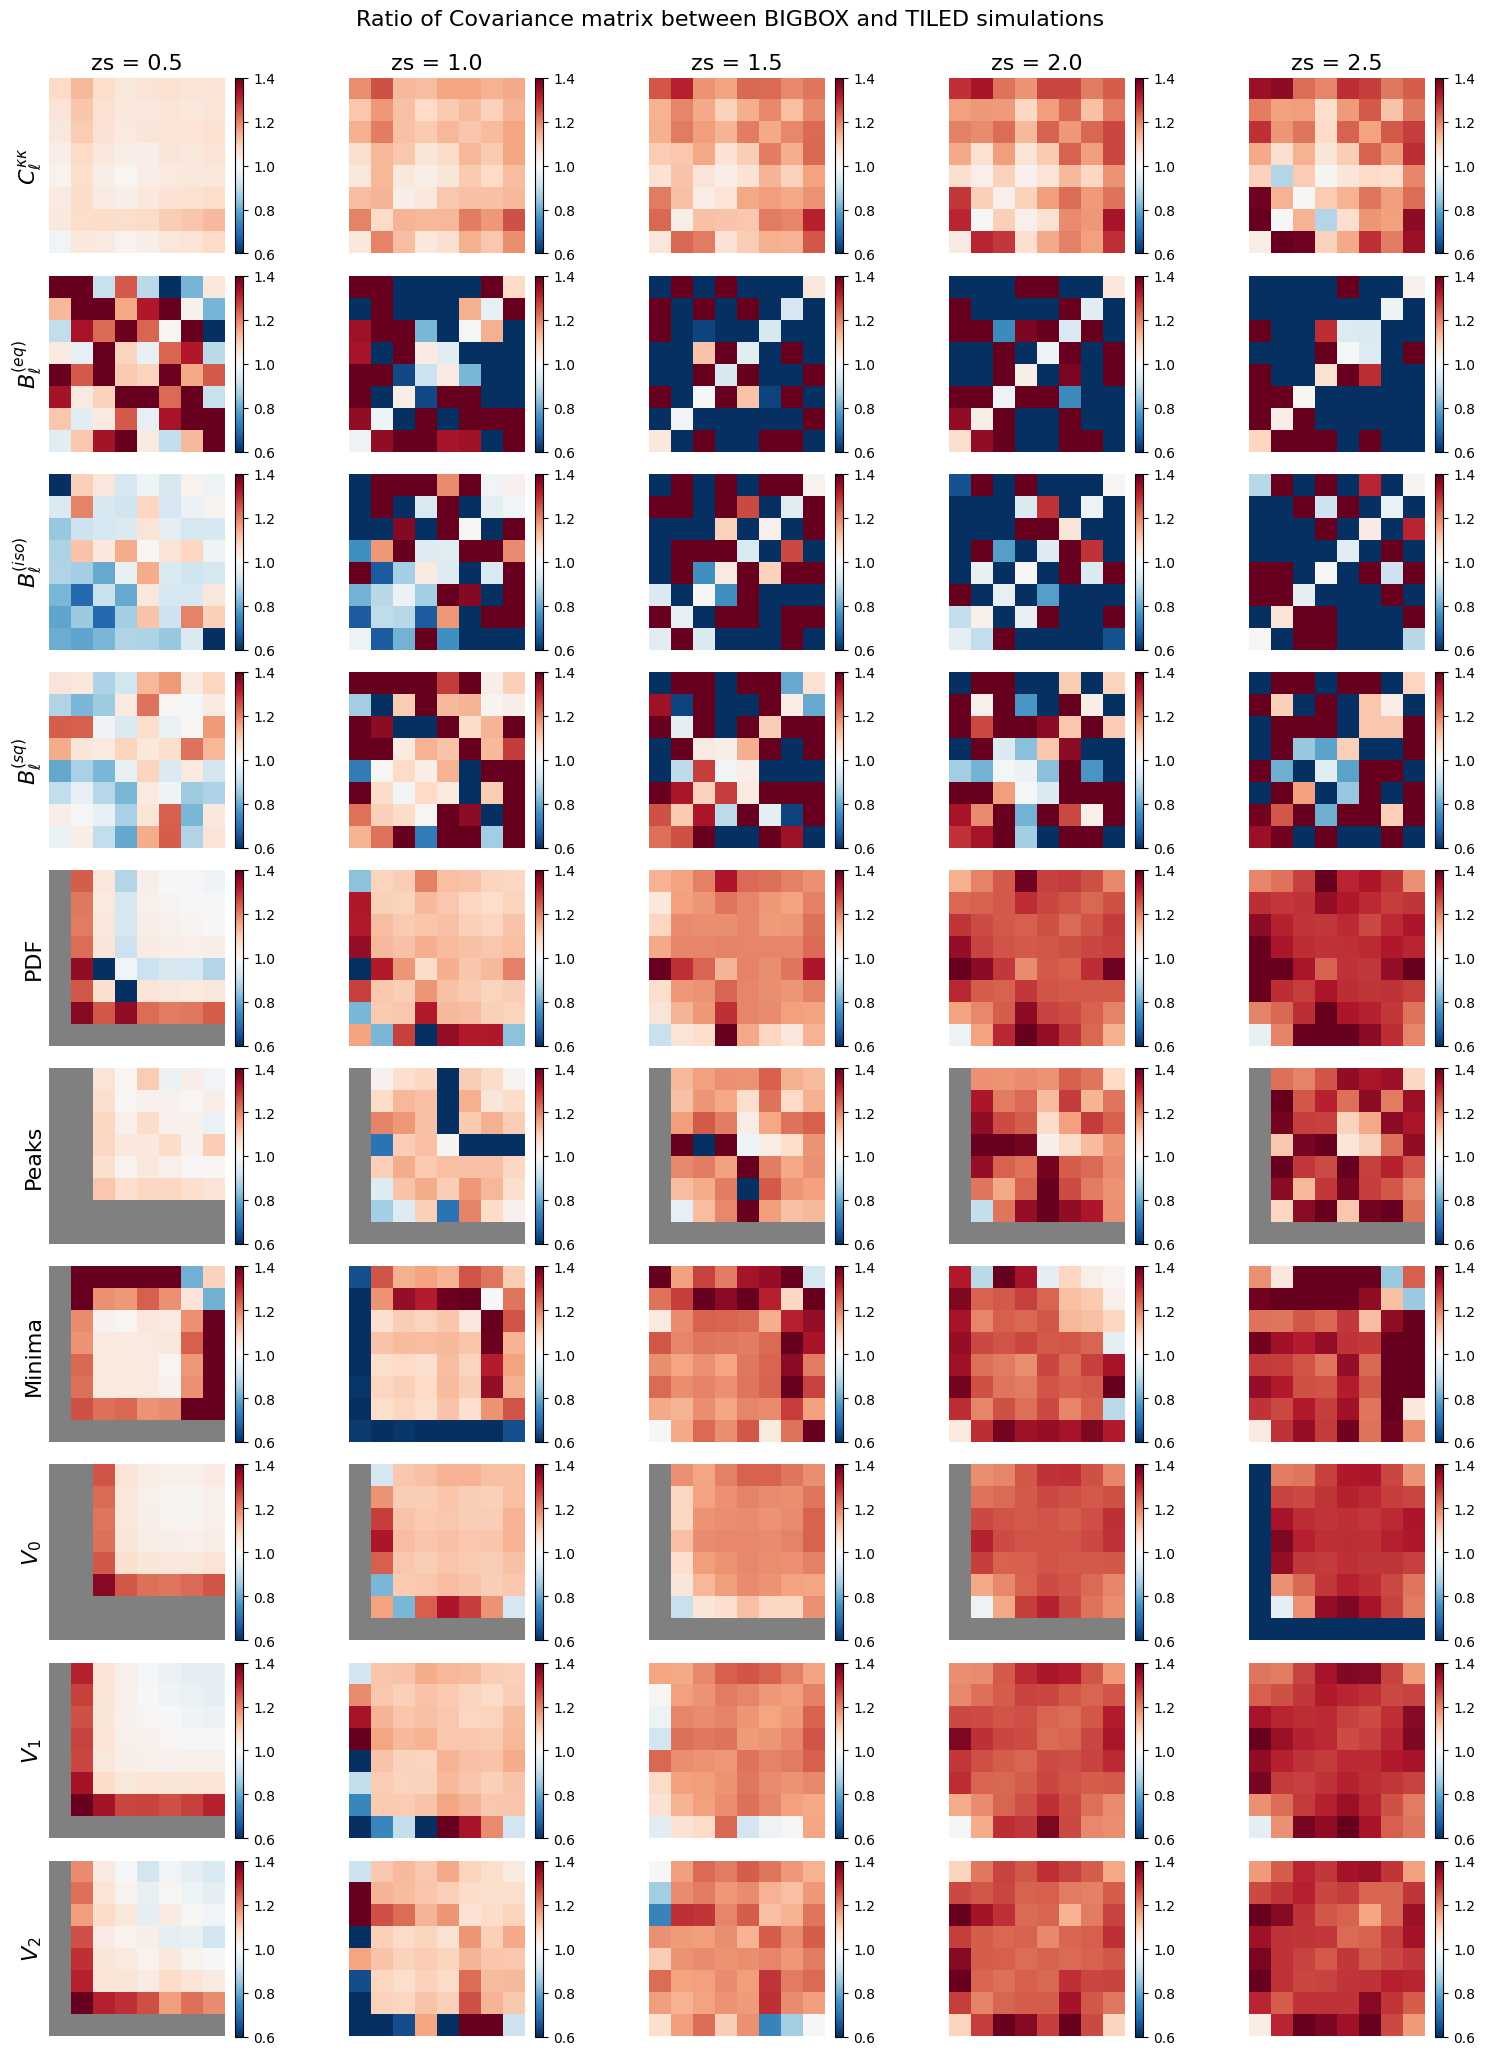
\includegraphics[width=\textwidth]{figures/results/cov_ratio.png}
    \caption[Ratios of Covariance Matrices between BIGBOX and TILED Simulations]{Ratios of covariance matrices between the BIGBOX and TILED simulations for multiple source redshifts. The ratios are consistently $10\%$ to $30\%$ higher than unity for most statistics, indicating the impact of super-sample covariance on the covariance structures.}
    \label{fig:cov_ratio_main}
\end{figure}

\begin{figure}[p]
    \centering
    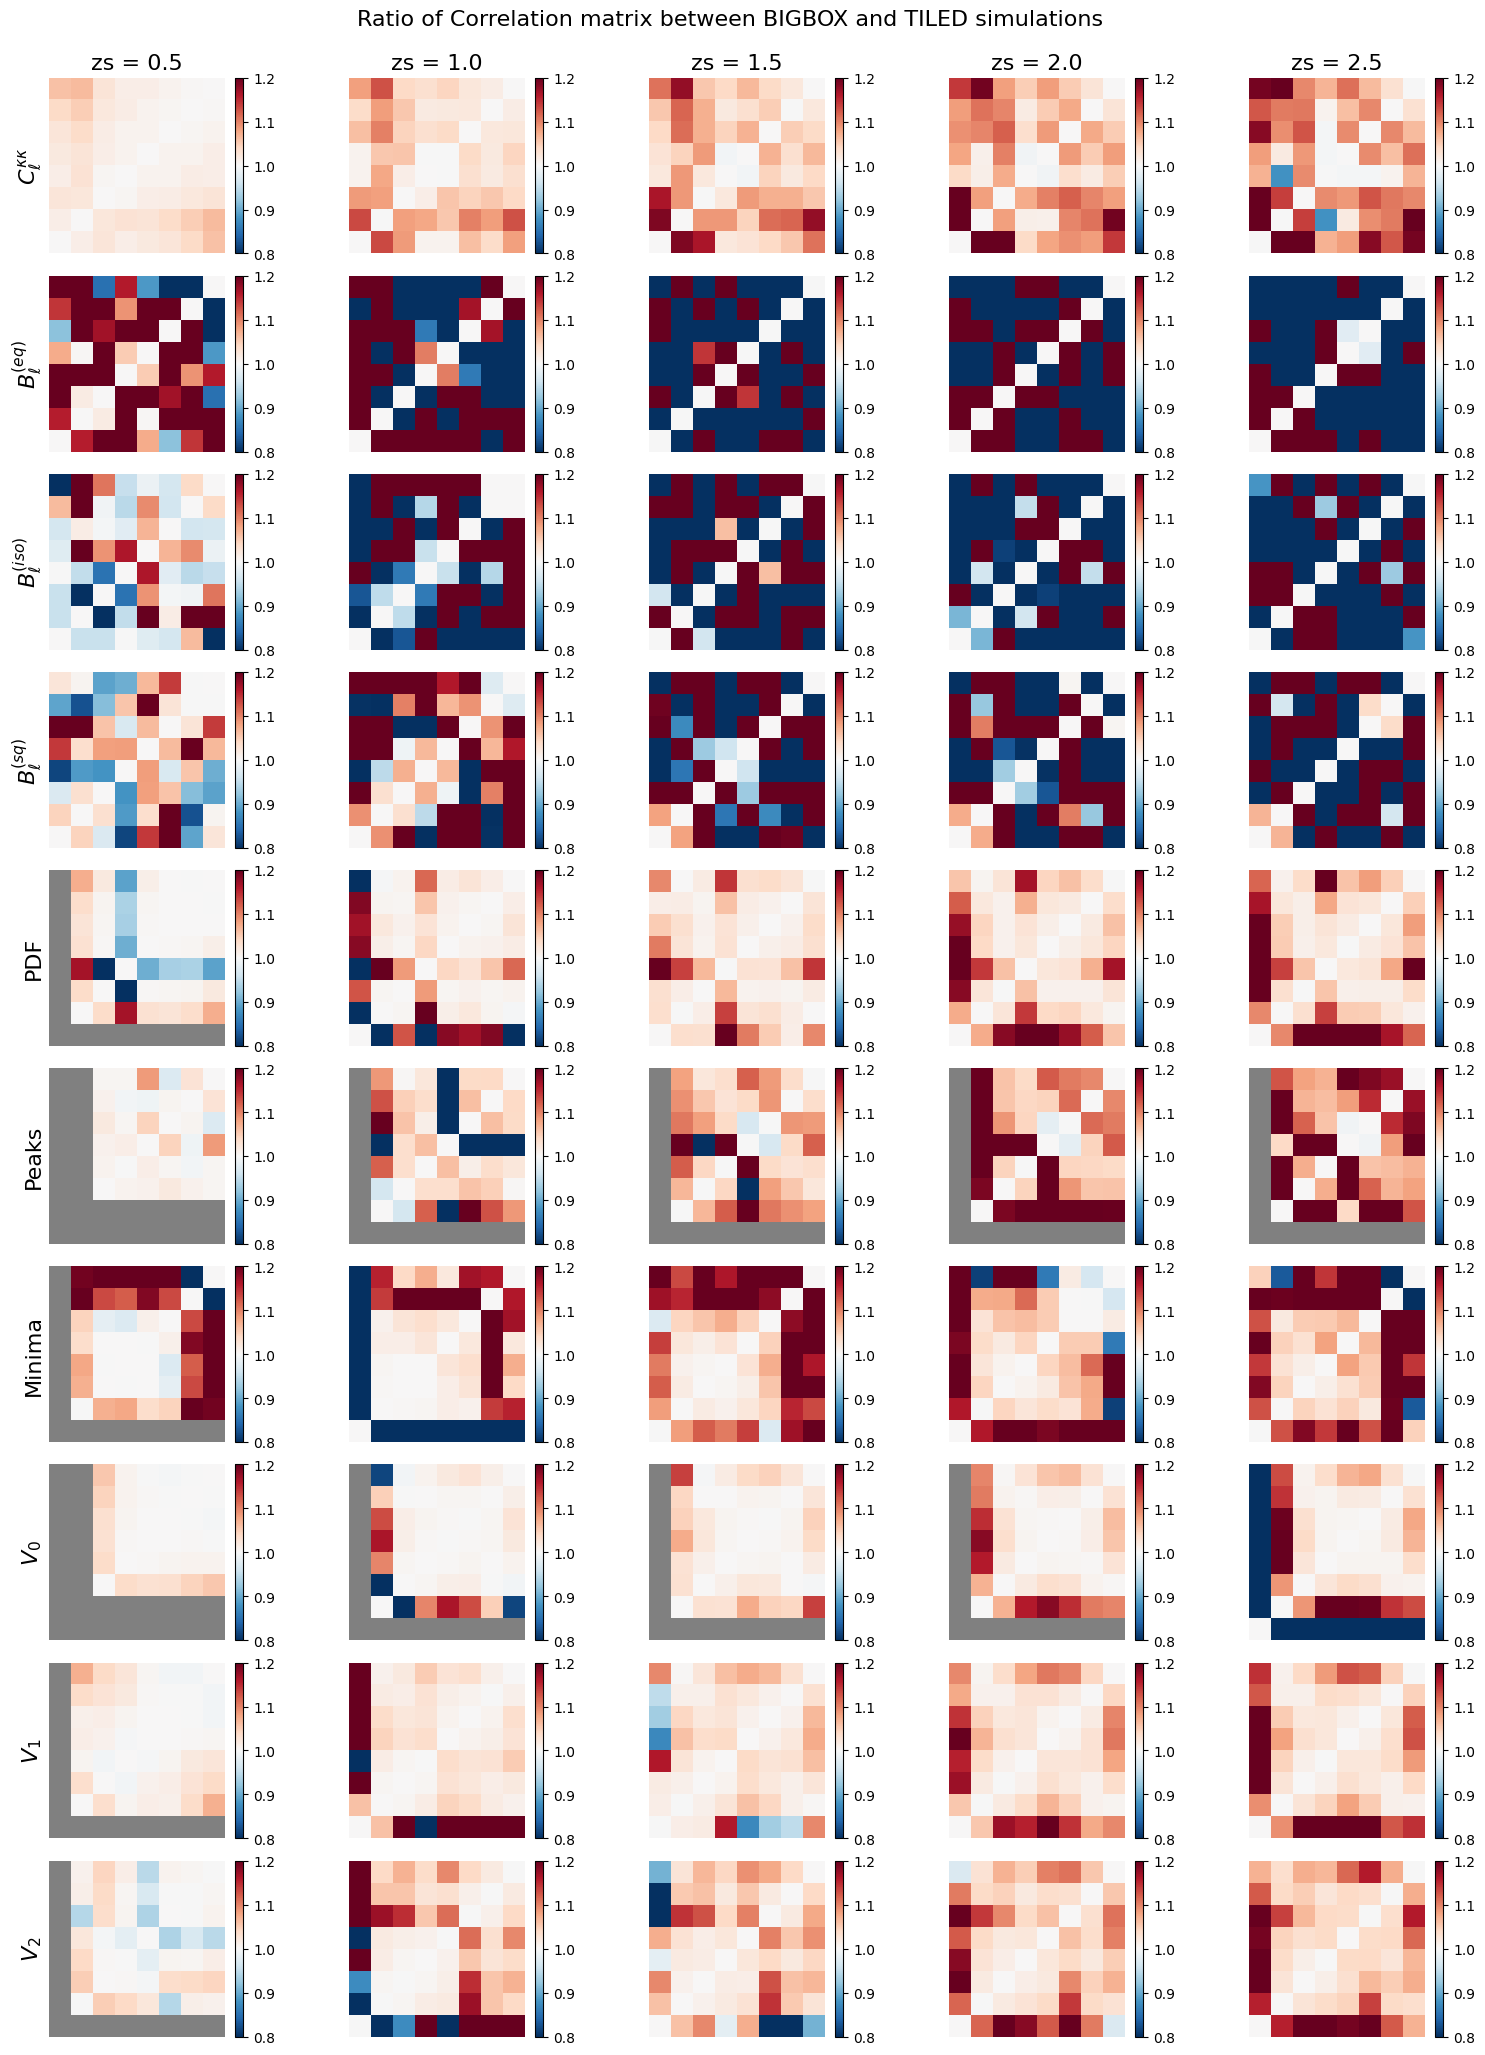
\includegraphics[width=\textwidth]{figures/results/corr_ratio.png}
    \caption[Ratios of Correlation Matrices between BIGBOX and TILED Simulations]{Ratios of correlation matrices between the BIGBOX and TILED simulations for multiple source redshifts. The ratios are generally $ < 5\%$, indicating that the super-sample effect is not only in the diagonal terms but also in the off-diagonal terms, lifting the overall covariance matrix.}
    \label{fig:corr_ratio_main}
\end{figure}

\clearpage

\section{Effects of Noise on Statistical Measures}
The presence of shape noise in convergence maps can significantly affect the covariance and correlation structures of statistical measures. To evaluate the effect between shape noise and super-sample effects, we applied several noise levels corresponding to current and future surveys (refer to Table~\ref{tab:survey_comparison}). This analysis seeks to determine the extent to which the super-sample effect remains dominant over the noise contribution. Given that the bispectrums already have no clear trends in the noiseless case (as shown in Figures~\ref{fig:cov_ratio_main} and~\ref{fig:corr_ratio_main}), we focus primarily on the angular power spectrum and other higher-order statistics.

Figures~\ref{fig:avg_cov_noise} and~\ref{fig:cov_noise} present the ratios of covariance matrices and their averages for the statistical measures between the BIGBOX and TILED simulations at various noise levels. While the angular power spectrum and peak/minima counts exhibit greater sensitivity to noise, particularly at high noise levels (e.g., DES and HSC scenarios), the increasing trend of covariance ratios persists across most statistics. This suggests that for future surveys, the super-sample effect will likely dominate over the noise contribution.

In contrast, Figures~\ref{fig:avg_corr_noise} and~\ref{fig:corr_noise} show the ratios of correlation matrices and their averages for the statistical measures at different noise levels. Here, the ratios generally remain below $10\%$ for most statistics, indicating that noise does not drastically alter the overall structure of the covariance matrix. Higher values in the correlation ratios are primarily localized at the edges of each statistical measure. These high ratios arise from regions where the number of data points is sparse, making the measurements more susceptible to noise amplification. 

\begin{figure}[p]
    \centering
    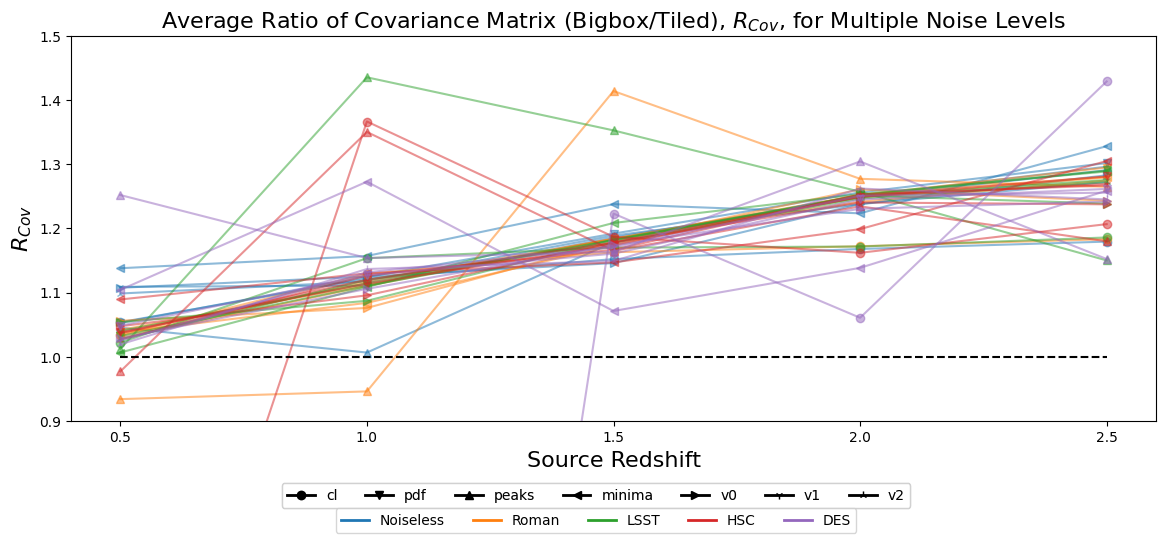
\includegraphics[width=0.95\textwidth]{figures/results/avg_cov_ratio_noise.png}
    \caption[Average BIGBOX/TILED Ratio of Covariance for Multiple Noise Levels]
    {Average ratio of covariance matrices for statistical measures between the BIGBOX and TILED simulations at different shape noise levels (refer to Table~\ref{tab:survey_comparison}). While the angular power spectrum and peak/minima counts exhibit higher sensitivity to noise variations, particularly under high noise levels, the overall increasing trend in covariance ratios persists across most statistical measures.}
    \label{fig:avg_cov_noise}
    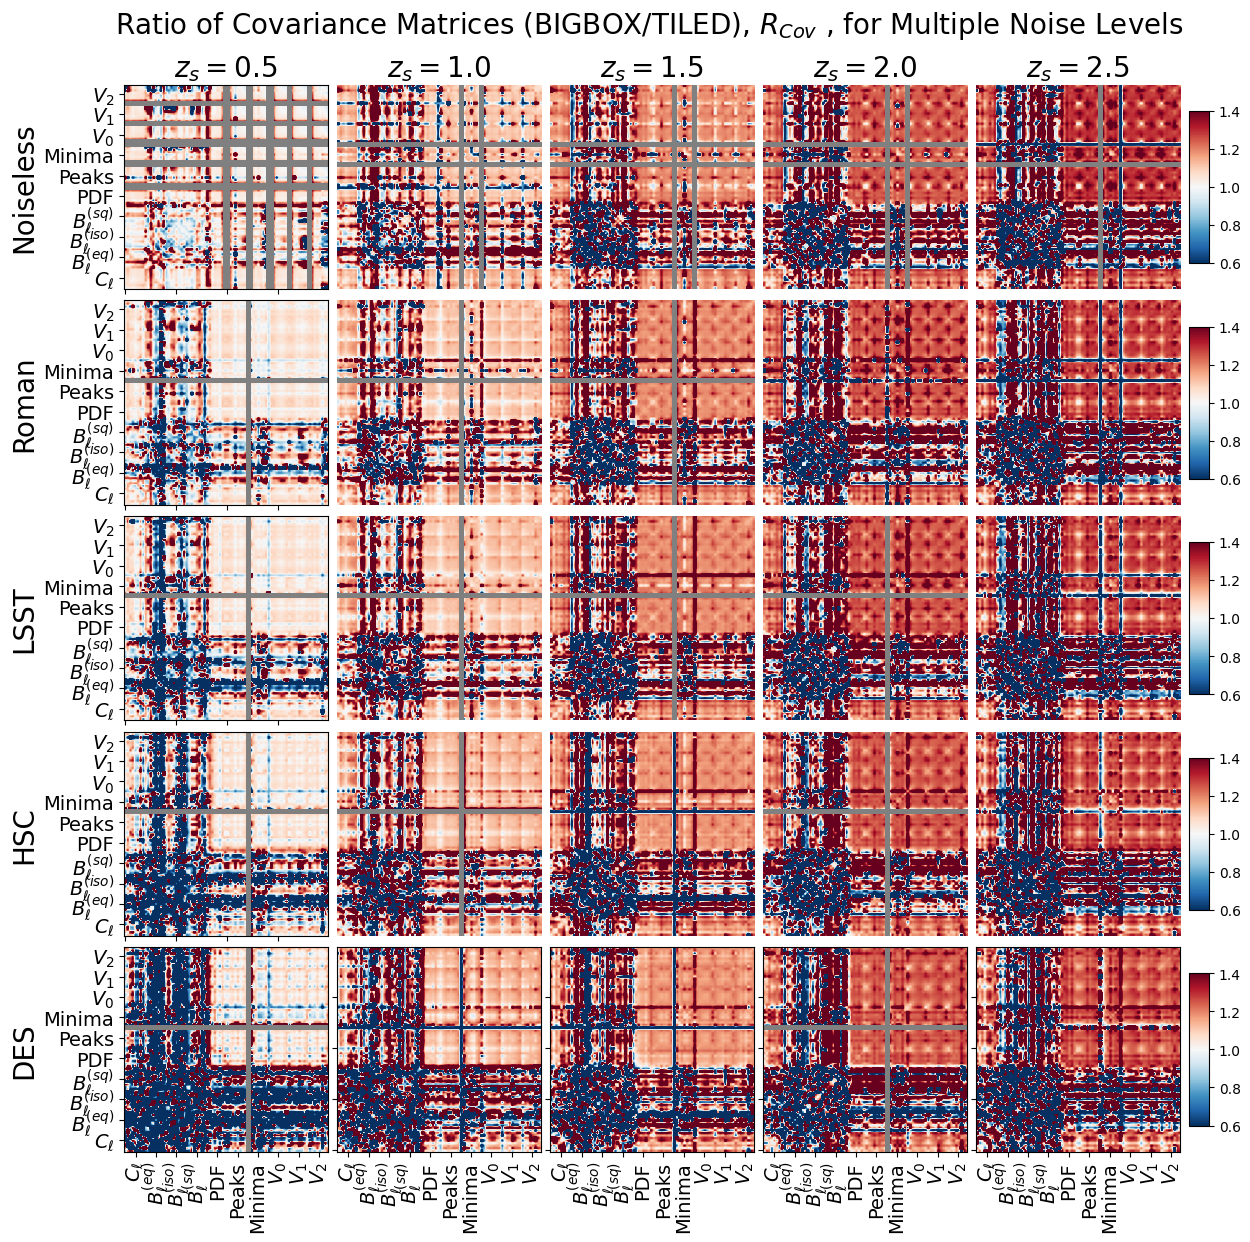
\includegraphics[width=0.95\textwidth]{figures/results/cov_noise.png}
    \caption[BIGBOX/TILED Ratio of Covariance for Multiple Noise Levels]
    {Ratio of covariance matrices for statistical measures between the BIGBOX and TILED simulations at varying shape noise levels. Despite the bispectrum, the covariance ratio structure maintains a consistent increasing trend, suggesting the sustained influence of super-sample covariance across different noise conditions.}
    \label{fig:cov_noise}
\end{figure}

\begin{figure}[p]
    \centering
    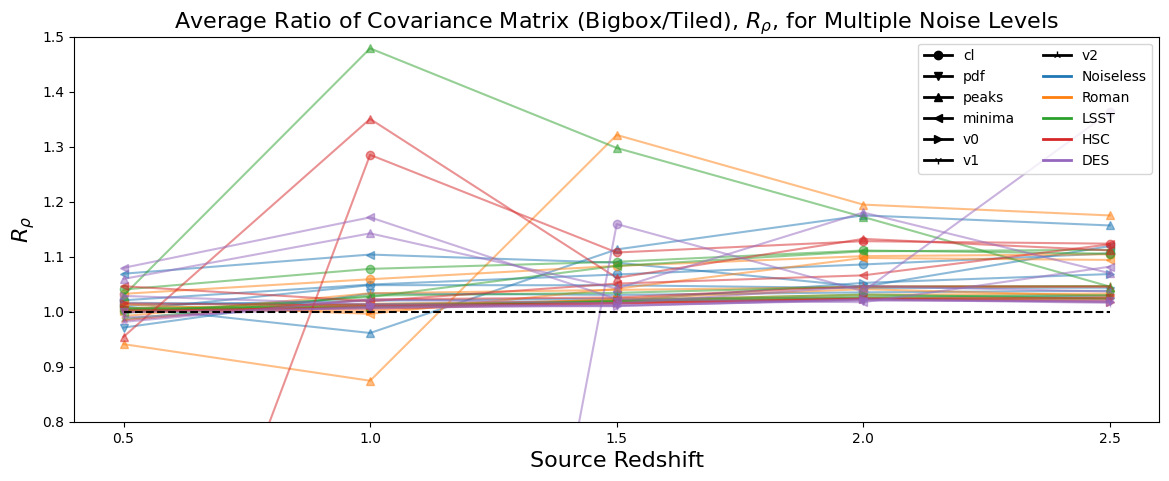
\includegraphics[width=0.95\textwidth]{figures/results/avg_corr_ratio_noise.png}
    \caption[Average BIGBOX/TILED Ratio of Correlation for Multiple Noise Levels]
    {Average ratio of correlation matrices for statistical measures between the BIGBOX and TILED simulations at varying shape noise levels (see Table~\ref{tab:survey_comparison}). While the angular power spectrum and peak counts display higher sensitivity to noise, the overall correlation ratios remain below $10\%$ for most statistics.}
    \label{fig:avg_corr_noise}
    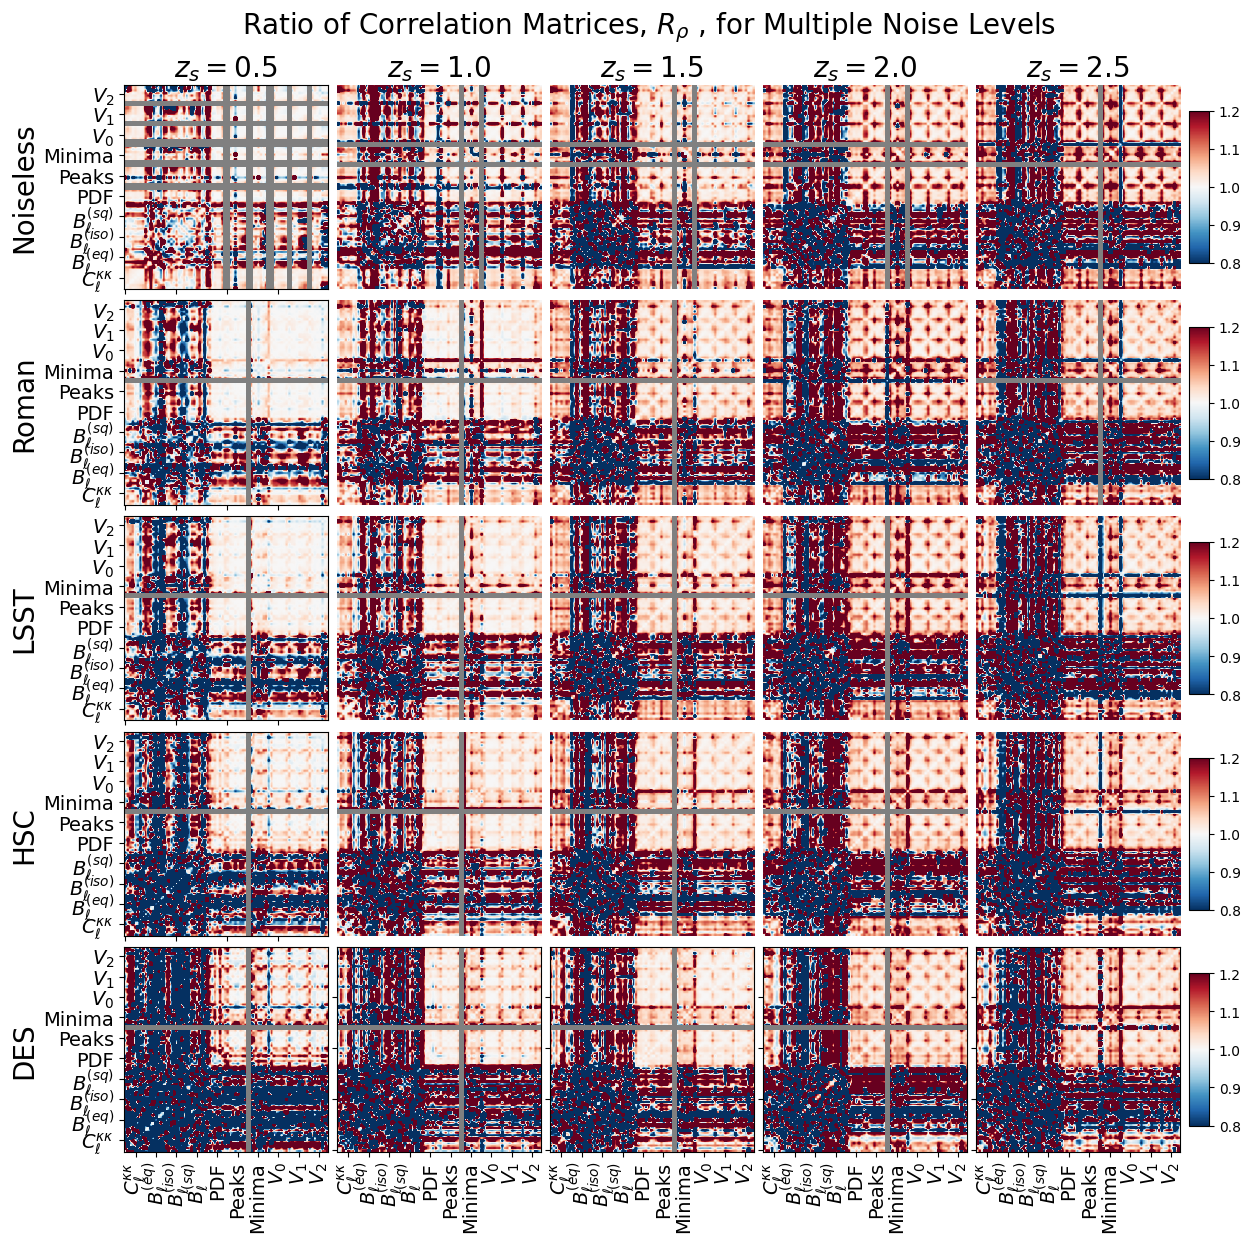
\includegraphics[width=0.95\textwidth]{figures/results/corr_noise.png}
    \caption[BIGBOX/TILED Ratio of Correlation for Multiple Noise Levels]
    {Ratio of correlation matrices for statistical measures between the BIGBOX and TILED simulations at different shape noise levels. High correlation ratios primarily occur at the edges of the statistical measures, where sparse data and amplified noise dominate. }
    \label{fig:corr_noise}
\end{figure}

\clearpage

\section{Influence of Smoothing Scale}
We analyze the impact of varying Gaussian smoothing scales on the statistical measures, focusing on how smoothing modifies the underlying structures in convergence maps. As the smoothing scale increases, small-scale features are progressively suppressed, leading to a redistribution of signal intensities. Notably, smoothed convergence maps were not utilized for the calculation of the angular power spectrum and bispectrum; thus, the results are presented exclusively for other higher-order statistics.

Figures~\ref{fig:avg_cov_sl} and~\ref{fig:cov_smoothing} depict the changes in the ratios of covariance matrices and their averages as a function of the smoothing scale. Across all smoothing scales, the average covariance ratios between the BIGBOX and TILED simulations exhibit a consistent upward trend for most statistical measures. However, notable variations are observed in the peak/minima counts, particularly at larger smoothing scales. These variations are attributed to the averaging methodology, where contributions from the edges of $\nu$ bins and peak bins become increasingly significant at higher smoothing levels.

Figures~\ref{fig:avg_corr_sl} and~\ref{fig:corr_smoothing} show the corresponding ratios of correlation matrices and their averages for different smoothing scales. The correlation ratios generally remain below $5\%$ for most statistics, suggesting that the overall structure of the covariance matrix is robust to variations in smoothing scale. However, similar to the covariance trends, peak/minima counts exhibit elevated correlation ratios,  especially at larger smoothing scales.

In summary, the findings suggest that while Gaussian smoothing scales can influence individual statistical measures, the overall structural integrity of the covariance and correlation matrices remains largely unaffected by changes in the smoothing scale.

\begin{figure}[p]
    \centering
    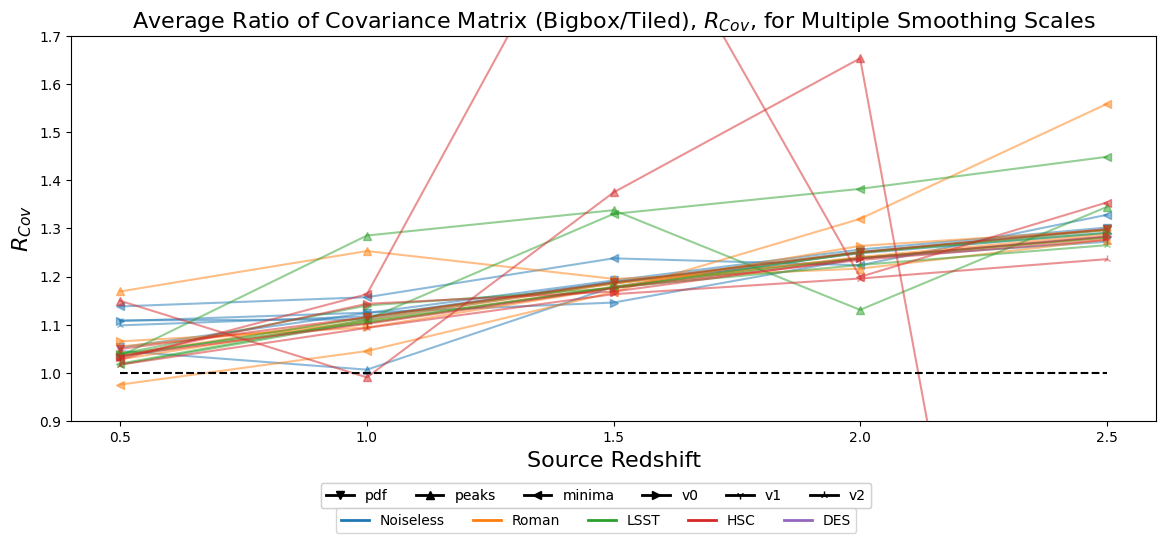
\includegraphics[width=\textwidth]{figures/results/avg_cov_ratio_sl.png}
    \caption[Average BIGBOX/TILED Ratio of Covariance for Multiple Smoothing Scales]
    {Average ratio of covariance matrices for various statistical measures between the BIGBOX and TILED simulations at differing Gaussian smoothing scales. The overall increasing trend in covariance ratios persists across all smoothing scales, with pronounced variations observed in peak and minima counts, particularly at larger smoothing scales where edge contributions in $\nu$ bins become more significant.}
    \label{fig:avg_cov_sl}
    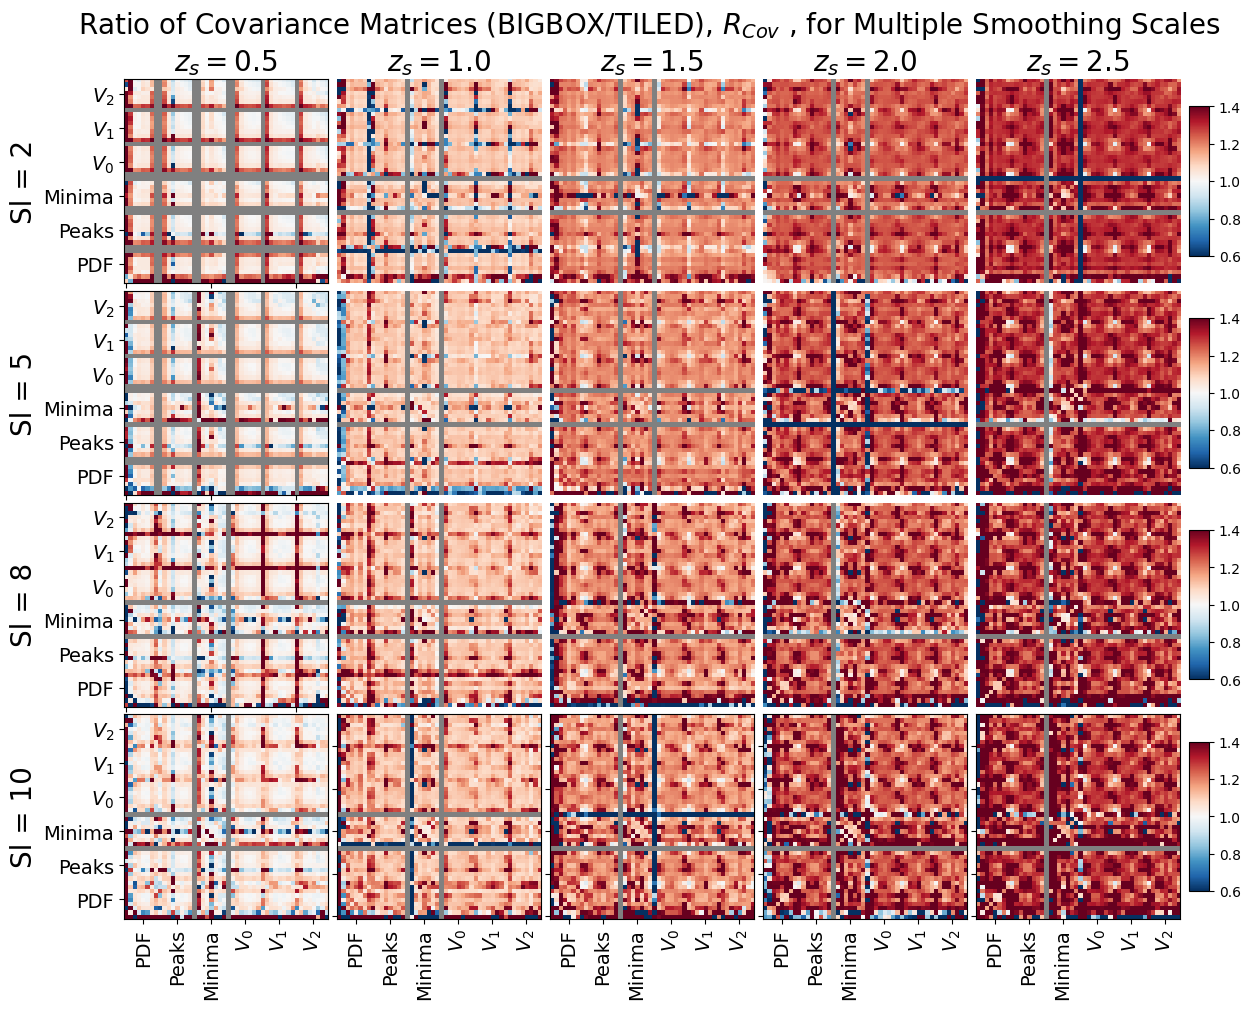
\includegraphics[width=\textwidth]{figures/results/cov_smoothing.png}
    \caption[BIGBOX/TILED Ratio of Covariance for Multiple Smoothing Scales]
    {Ratio of covariance matrices for various statistical measures between the BIGBOX and TILED simulations across different Gaussian smoothing scales. The covariance ratios exhibit consistent trends regardless of the smoothing scale applied.}
    \label{fig:cov_smoothing}
\end{figure}

\begin{figure}[p]
    \centering
    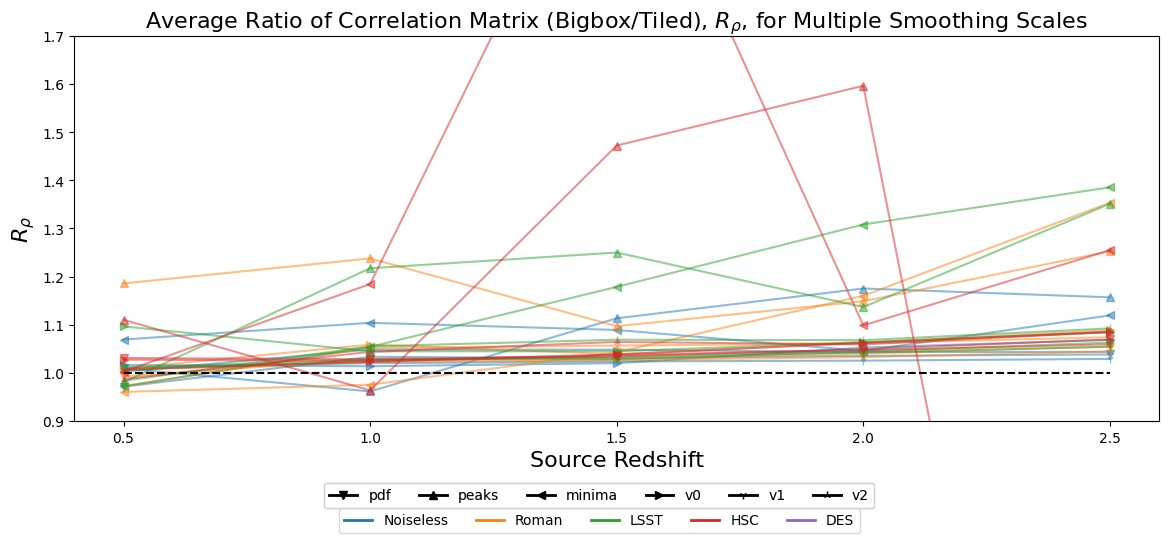
\includegraphics[width=\textwidth]{figures/results/avg_corr_ratio_sl.png}
    \caption[Average BIGBOX/TILED Ratio of Correlation for Multiple Smoothing Scales]
    {Average ratio of correlation matrices for various statistical measures between the BIGBOX and TILED simulations at different Gaussian smoothing scales. Correlation ratios predominantly remain below $5\%$ for most metrics, underscoring the minimal impact of smoothing on the overall covariance matrix structure. Peak and minima counts, however, exhibit greater variations at higher smoothing scales due to the increased influence of edge contributions in $\nu$ bins.}
    \label{fig:avg_corr_sl}
    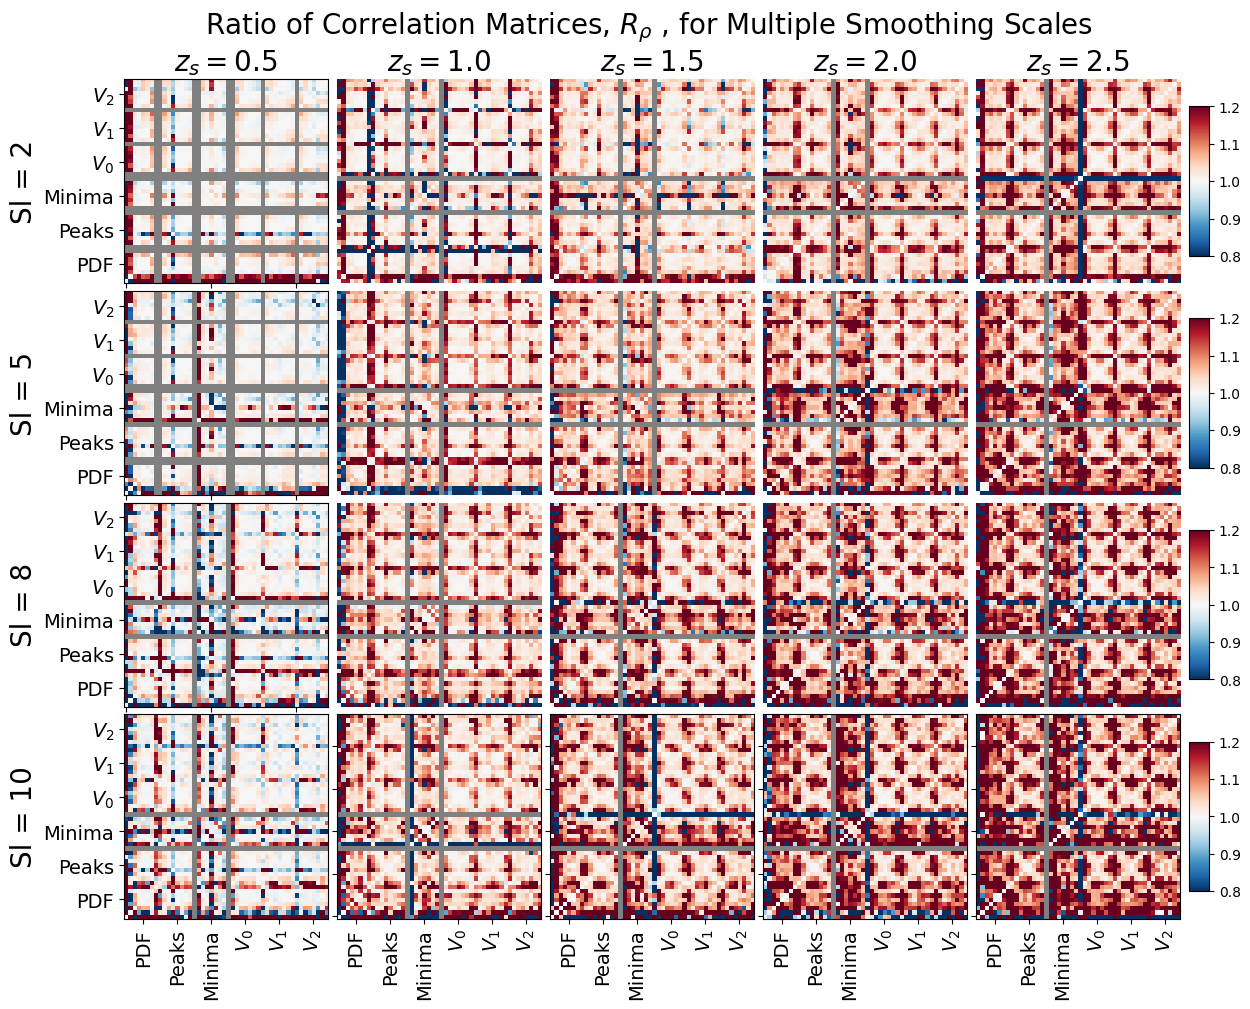
\includegraphics[width=\textwidth]{figures/results/corr_smoothing.png}
    \caption[BIGBOX/TILED Ratio of Correlation for Multiple Smoothing Scales]
    {Ratio of correlation matrices for various statistical measures between the BIGBOX and TILED simulations across different Gaussian smoothing scales. Except for the boundaries of $\nu$ bins, the correlation ratios remain modest across all smoothing scales.} 
    \label{fig:corr_smoothing}
\end{figure}

\clearpage

\section{Systematic Effects: Box Replication Artifact} \label{sec:boxreplication}
In weak lensing simulations, extending the simulated volume often necessitates the replication of simulation boxes. This box replication process can inadvertently introduce artificial correlations, particularly near the boundaries or along specific replication directions, thereby impacting the reliability of higher-order statistical measures. To systematically investigate this issue, we categorize simulation regions into \textbf{Replication-Influenced Patches (RIP)} and \textbf{Replication-Minimal Patches (RMP)} based on their susceptibility to replication-induced artifacts.
The criteria for categorizing patches are as follows:
\begin{itemize} 
    \item Replication-Influenced Patches (RIP):
    \begin{itemize}
        \item Patches near the equator: $ \left| \theta_i - \frac{\pi}{2} \right| \leq R_{\text{patch}} $ 
        \item Patches near the edges of octants: $ \left| \phi_i - \frac{k\pi}{2} \right| \leq R_{\text{patch}} $ for $k = 0, 1, 2, 3$
    \end{itemize}
    \item Replication-Minimal Patches (RMP):
    \begin{itemize}
        \item All other patches not meeting the above criteria.
    \end{itemize}
\end{itemize}
where $(\theta_i, \phi_i)$ denote the center of patch $i$, and $R_{\text{patch}} = 5\sqrt{2}\, \mathrm{\deg}$ is the half-diagonal of the patch.

Our analysis indicates that patches containing the point $(\theta_i, \phi_i) = (\pi/2, 0)$ exhibit significant deviations in both their mean and variance compared to other RIPs. To prevent these outliers from skewing our results, we exclude this specific point from subsequent analyses.

After these adjustments, we obtained $70$ RMP per realization, and $1400$ RMP for the TILED simulations and $770$ RMP for the BIGBOX simulations across all realizations.

Figure~\ref{fig:boxreplication_main} illustrates the ratios of mean and variance for various statistical measures between RIPs and RMPs. The analysis reveals that the mean angular power spectra in RIPs are systematically underestimated by approximately $0.5\%$. Additionally, the $\nu$-binned statistics display elevated mean values in low $\nu$ bins and reduced values in high $\nu$ bins. This pattern suggests that box replication accentuates both overdense and underdense regions, leading to more extreme convergence values. In the TILED simulations, the limited resolution for underdense regions causes the $\nu$-binned statistics to shift toward lower $\nu$ bins. On the other hand, the variance ratios approach unity, indicating that the box replication effect amplifies the variance to levels comparable with those observed in BIGBOX simulations. Notably, the dependence on source redshift is effectively nullified in RIPs, implying that box replication covers the super-sample variance. 

\begin{figure}[p] 
    \centering 
    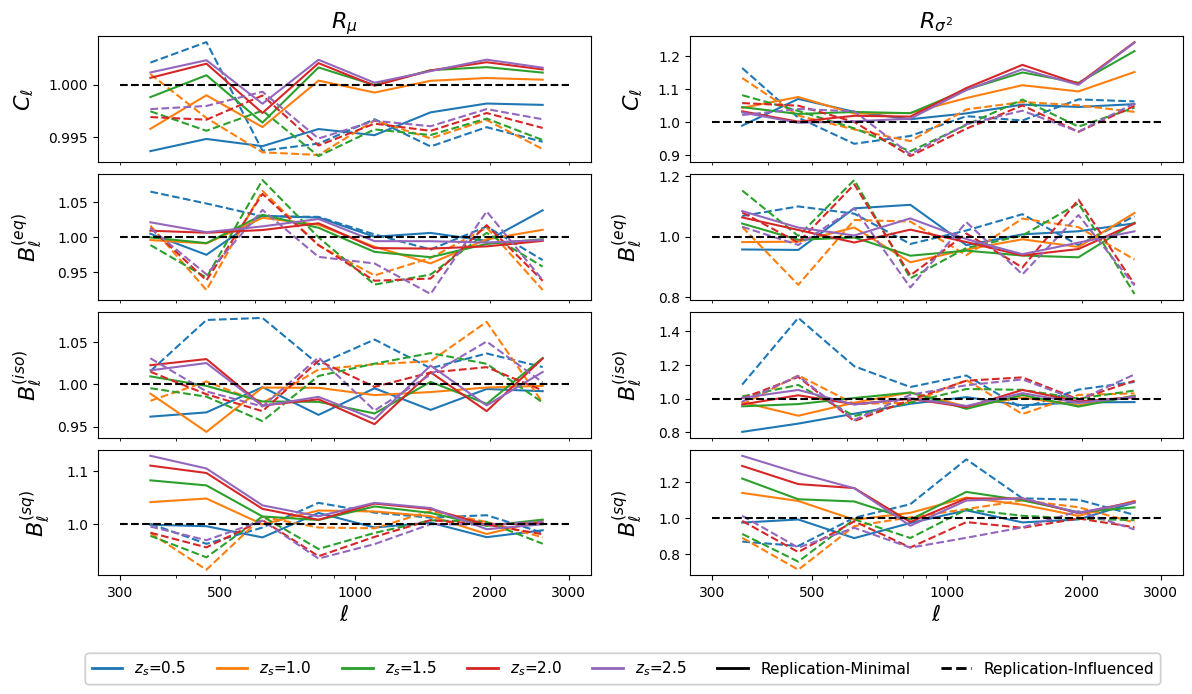
\includegraphics[width=\textwidth]{figures/results/BR_ratio_ell.png} 
    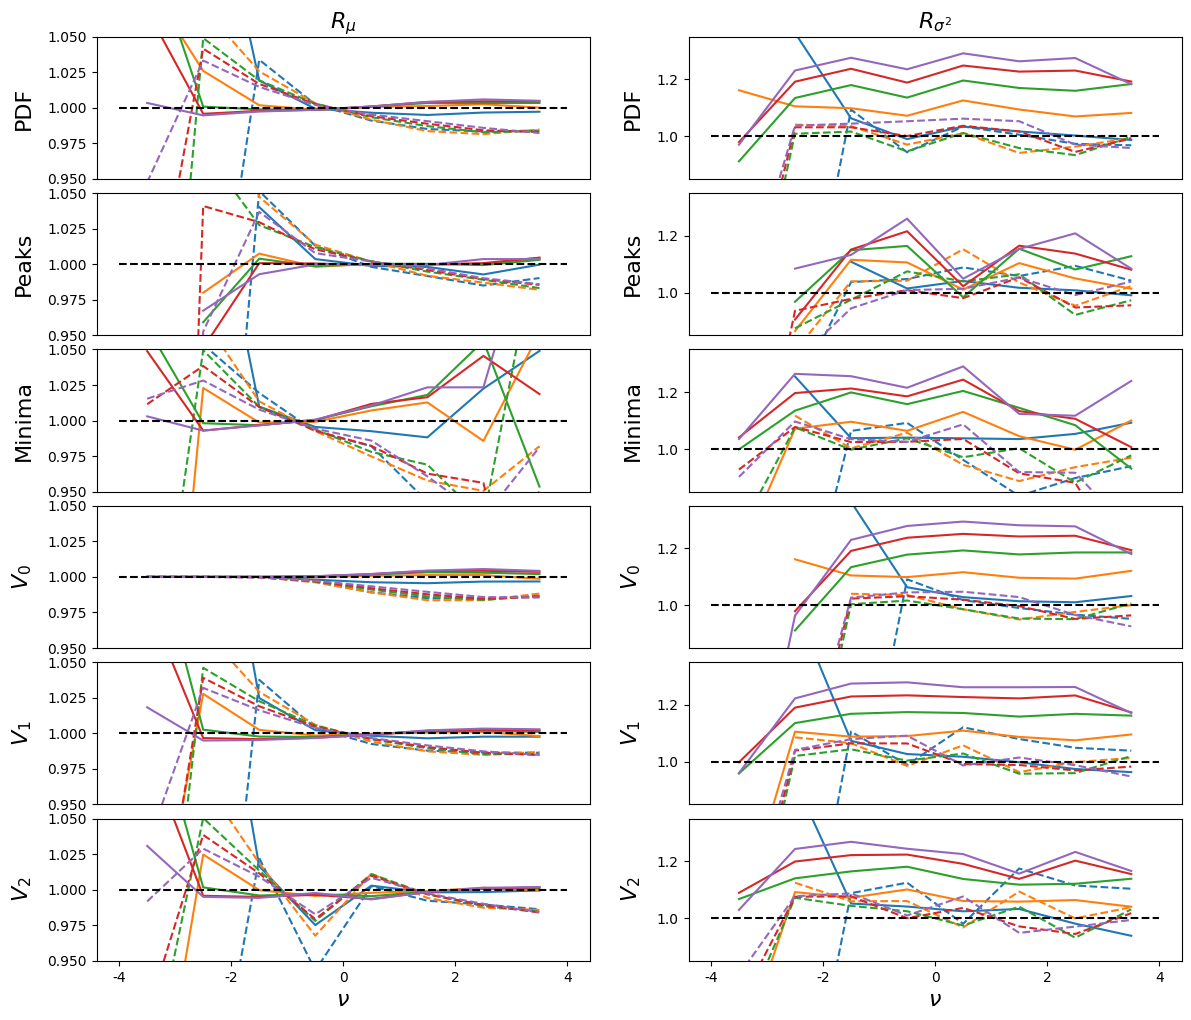
\includegraphics[width=\textwidth]{figures/results/BR_ratio_nu.png} 
    \caption[BIGBOX/TILED Ratios of the mean and variance of statistical measures for the RIPs and the RMPs]{Ratios of the mean and variance of statistical measures between Replication-Influenced Patches (RIP) and Replication-Minimal Patches (RMP). The $nu$-binned statistics show elevated means in low $nu$ bins and reduced means in high $nu$ bins. Variance ratios are generally close to unity, indicating that box replication amplifies the variance to levels comparable with BIGBOX simulations.} \label{fig:boxreplication_main} 
\end{figure}

Figures~\ref{fig:boxreplication_cov_RIP} and~\ref{fig:boxreplication_corr_RIP} display the ratios of covariance and correlation matrices between TILED and BIGBOX simulations for RIPs. Additionally, Figures~\ref{fig:boxreplication_avg_cov} and~\ref{fig:boxreplication_avg_corr} present the average ratios for both RIPs and RMPs. The main observations are that RIPs consistently exhibit lower covariance ratios compared to RMPs. Similarly, the correlation ratios for RIPs are generally lower than those for RMPs, except at $z_s=0.5$, where the super-sample effect is present in both TILED and BIGBOX simulations. Furthermore, distinct covariance structures, such as those for $C_\ell$ and $V_0$, emerge due to box replication artifacts. Structural transitions observed in previous analyses occur at higher redshifts ($z_s=2.0\sim2.5$) in RIPs, aligning with RMPs as higher redshift regions become dominated by RMPs.

\begin{figure}[ht]
    \centering
    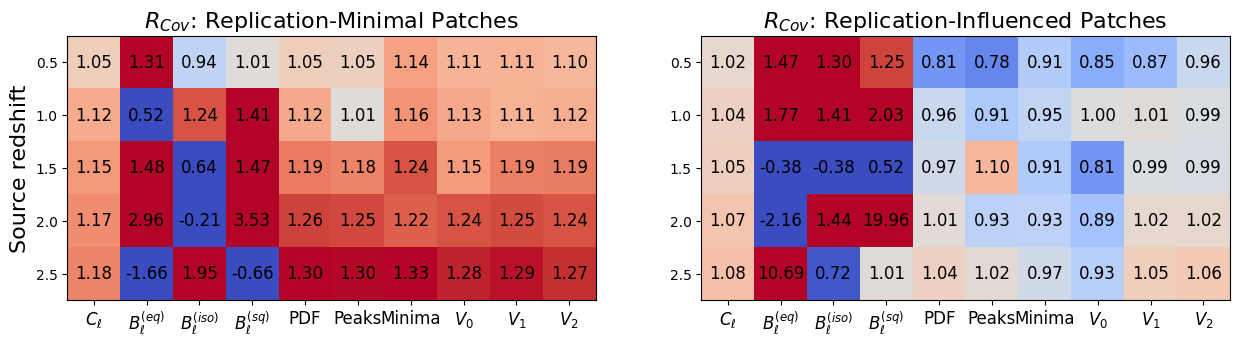
\includegraphics[width=\textwidth]{figures/results/BR_avg_cov_ratio.png}
    \caption[Average BIGBOX / TILED ratios of covariance matrices for the RIPs and the RMPs]{Average BIGBOX/TILED ratios of covariance matrices for Replication-Influenced Patches (RIP) and Replication-Minimal Patches (RMP). The ratios for RIPs (right panel) are consistently lower than those for RMPs (left panel), }
    \label{fig:boxreplication_avg_cov}
\end{figure}

\begin{figure}[ht]
    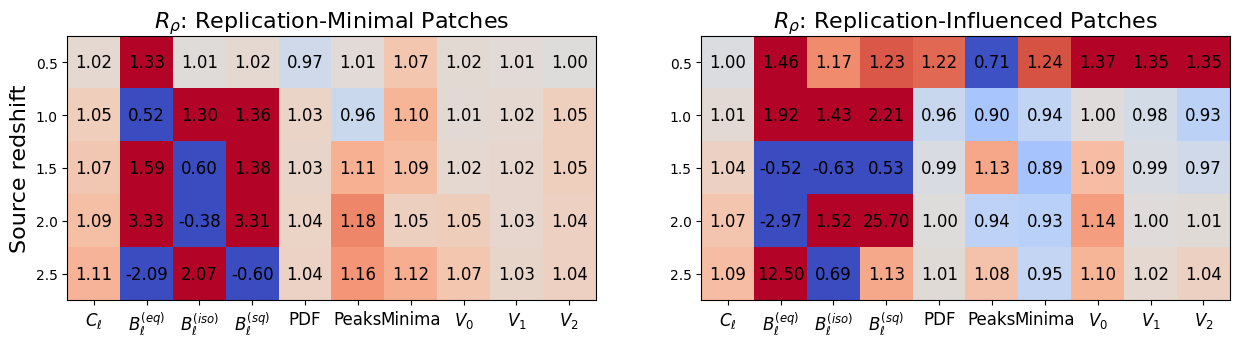
\includegraphics[width=\textwidth]{figures/results/BR_avg_corr_ratio.png}
    \caption[Average BIGBOX / TILED ratios of correlation matrices for the RIPs and the RMPs]{Average BIGBOX/TILED ratios of correlation matrices for Replication-Influenced Patches (RIP) and Replication-Minimal Patches (RMP). The ratios for RIPs (right panel) are consistently lower than those for RMPs (left panel), except at $z_s = 0.5$, where super-sample effects are present in both TILED and BIGBOX simulations.}
    \label{fig:boxreplication_avg_corr}
\end{figure}

\begin{figure}[p]
    \centering
    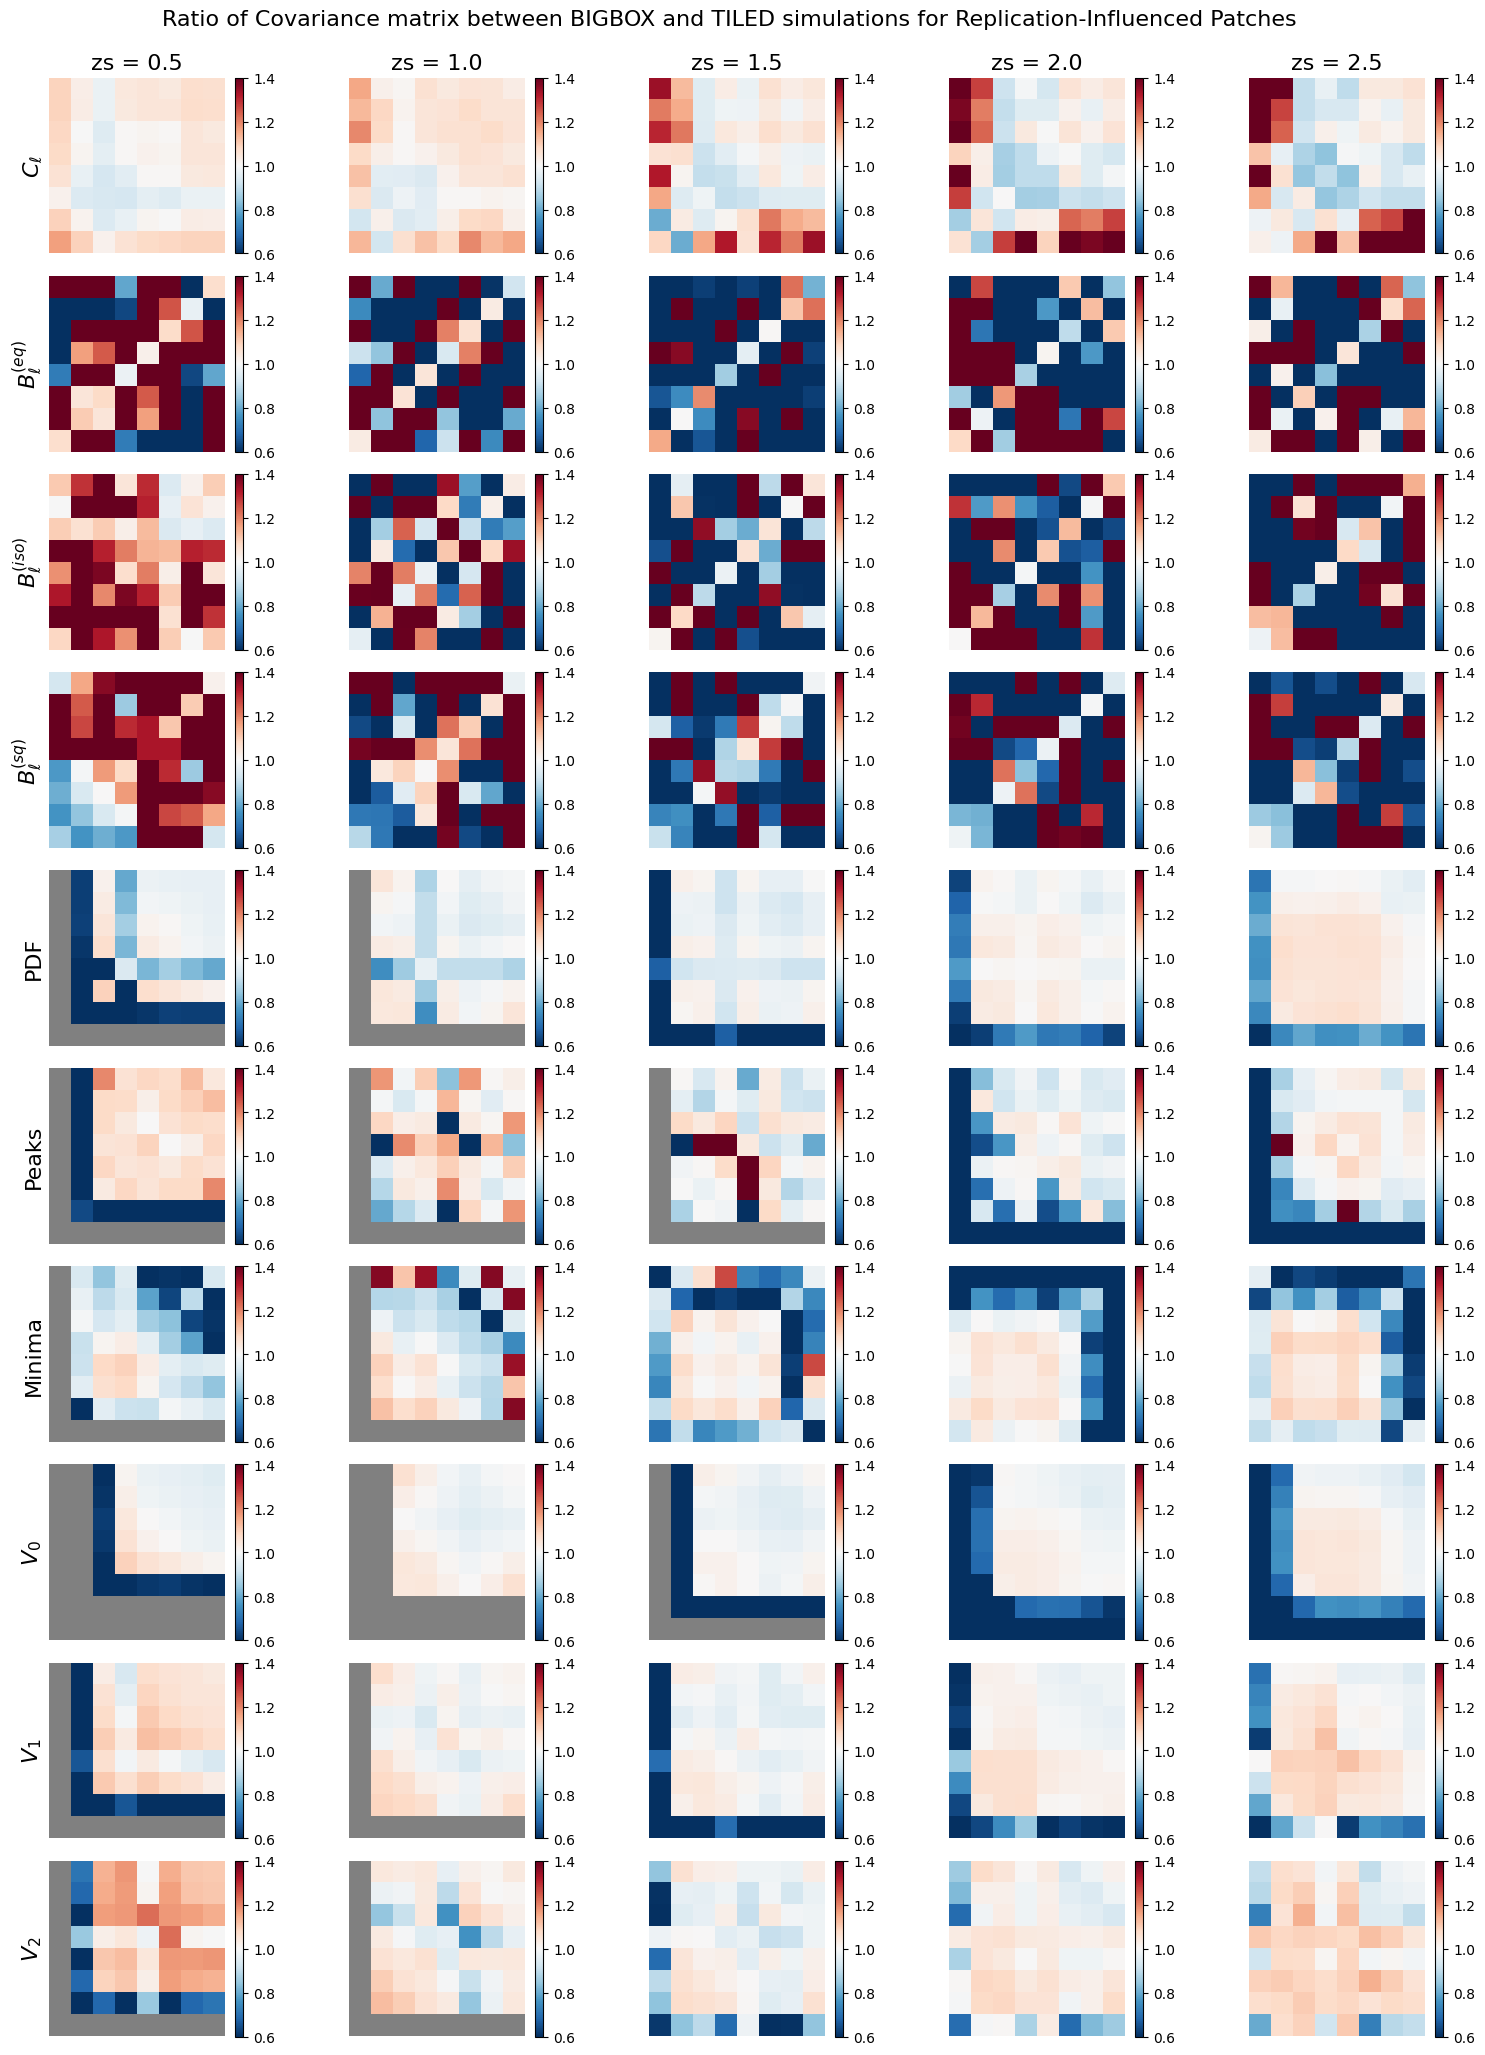
\includegraphics[width=\textwidth]{figures/results/cov_ratio_RIP.png}
    \caption[Covariance Ratios for RIP]{BIGBOX/TILED ratios of covariance matrices specifically for Replication-Influenced Patches (RIP). Compared to Figure~\ref{fig:corr_ratio_main}, RIP ratios are consistently lower than those for RMPs. Structures unique to RIPs, such as $C_\ell$ and $V_0$, indicate that box replication artifacts can generate distinct covariance structures.}
    \label{fig:boxreplication_cov_RIP}
\end{figure}

\begin{figure}[p]
    \centering
    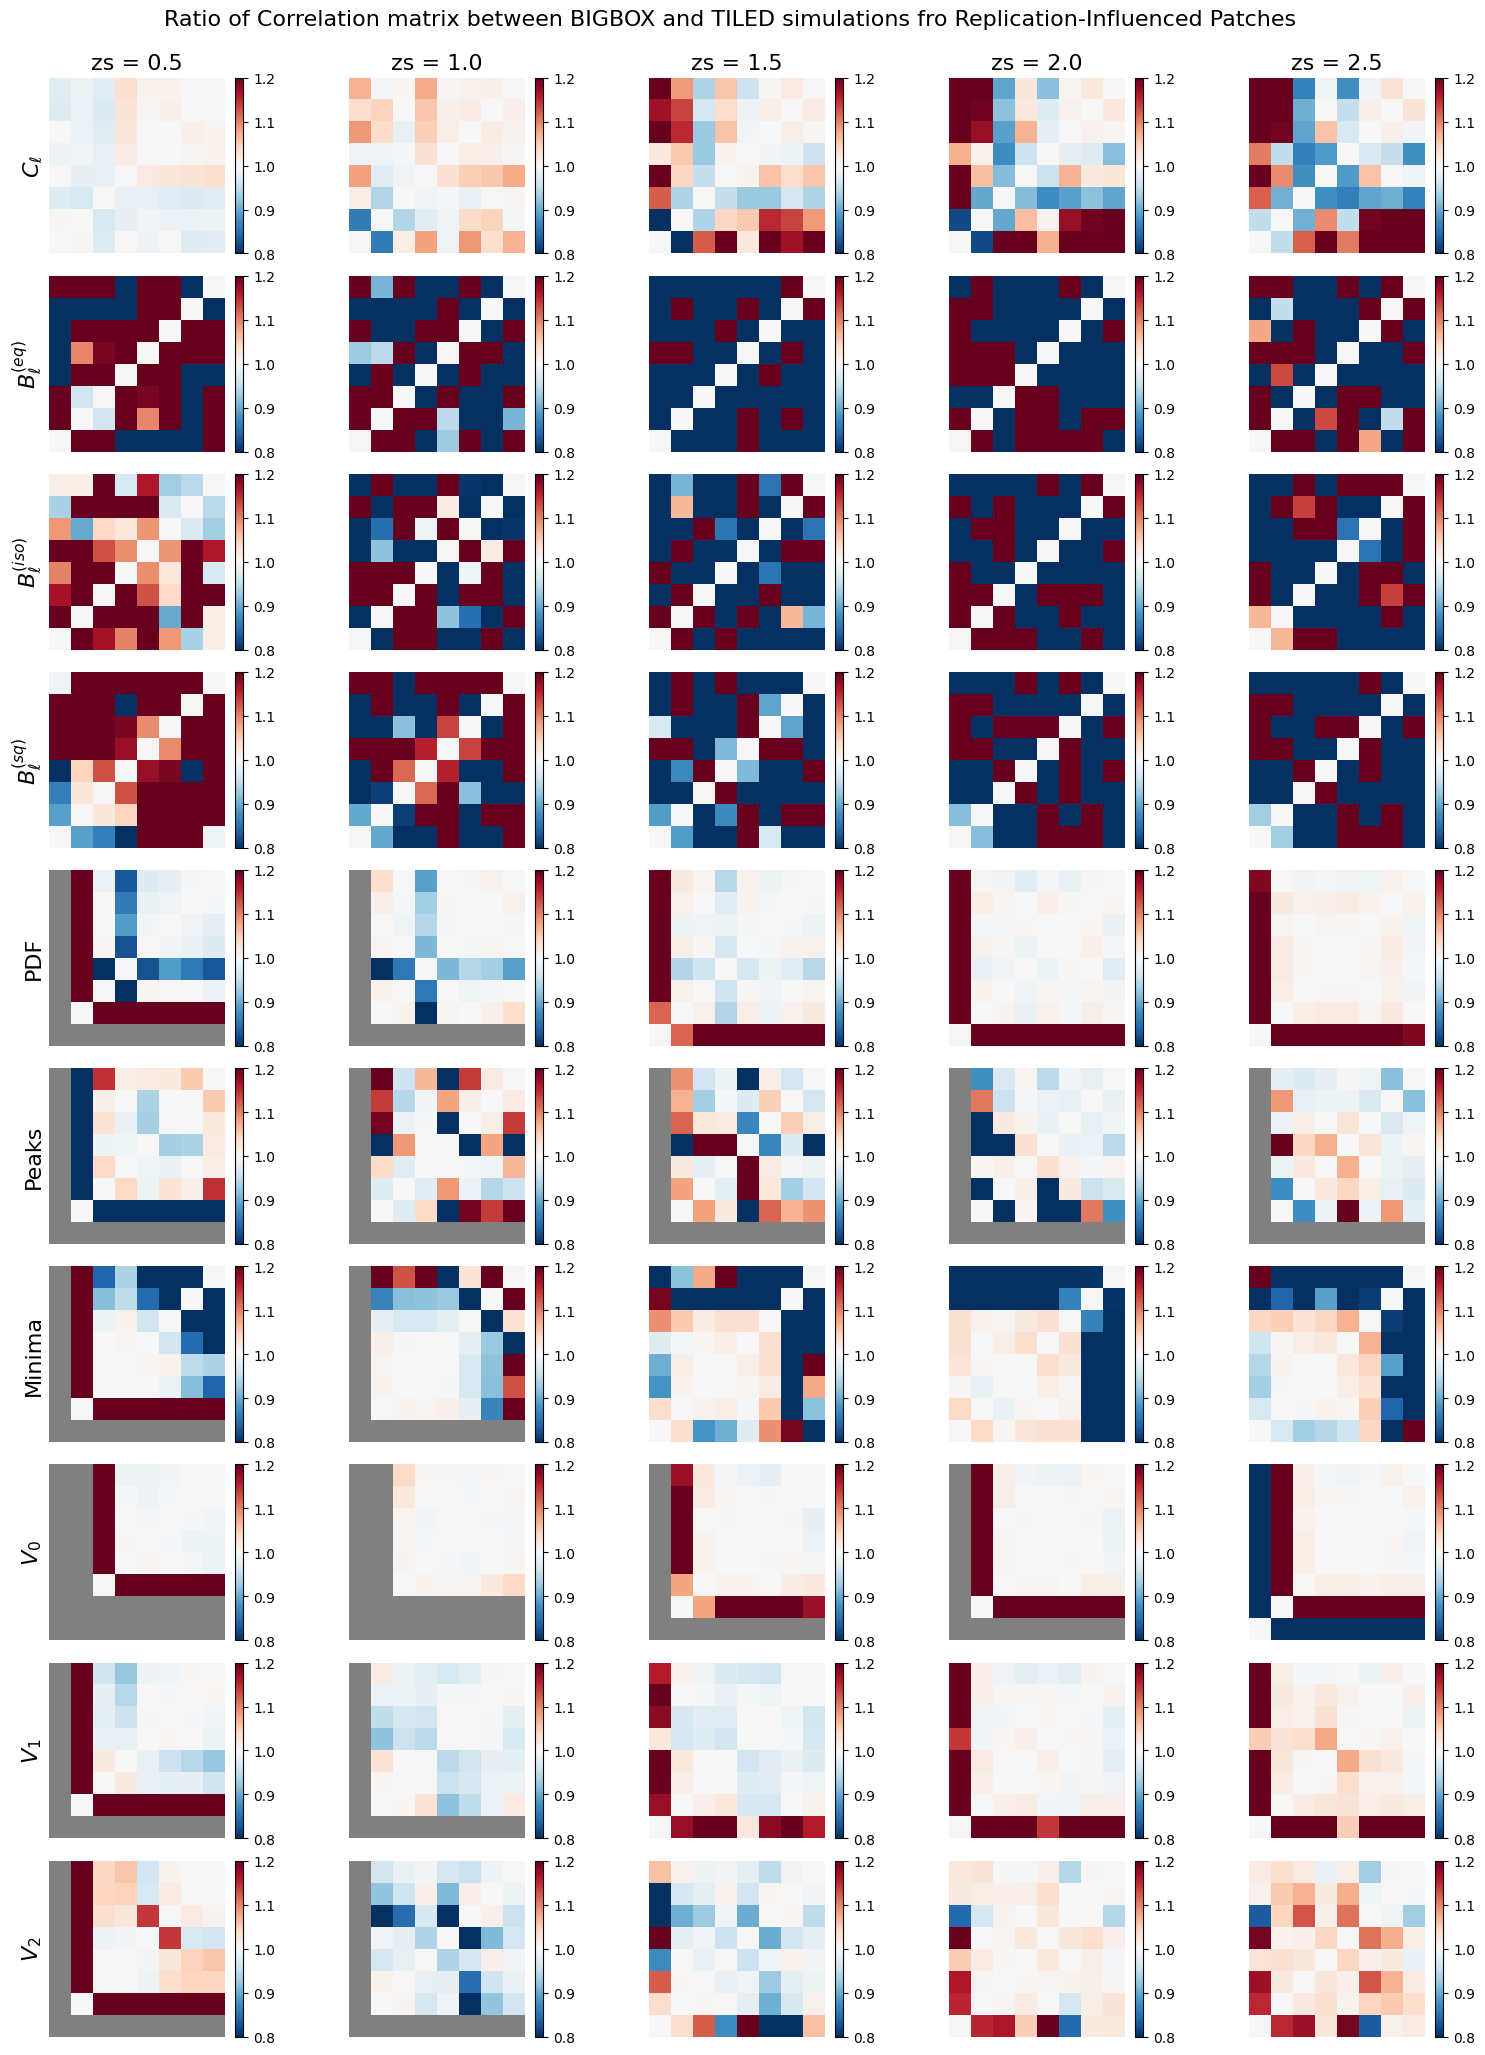
\includegraphics[width=\textwidth]{figures/results/corr_ratio_RIP.png}
    \caption[Correlation Ratios for RIP]{BIGBOX/TILED ratios of correlation matrices specifically for Replication-Influenced Patches (RIP). Similar to covariance ratios, RIP correlation ratios are consistently lower than those for RMPs. Off-diagonal structures are different from those in Figure~\ref{fig:corr_ratio_main} at lower redshifts, but they are likely to converge at higher redshifts.}
    \label{fig:boxreplication_corr_RIP}
\end{figure}

\clearpage

\section{Discussion}
Our findings confirm that the super-sample covariance effect significantly influences the covariance and correlation structures of higher-order weak lensing statistics. The mean values of statistical measures derived from the BIGBOX and TILED simulations exhibit remarkable consistency, with deviations typically below $1\%$. However, the variances of these measures demonstrate more pronounced differences, particularly at high $\ell$ and $\nu$ bins. The increasing trend in variance ratios with higher source redshifts underscores the progressive loss of large-scale modes in the TILED simulations, highlighting the impact of super-sample covariance on higher-order statistics. The covariance and correlation matrices further reveal the influence of super-sample covariance on both diagonal and off-diagonal elements, with the covariance ratios consistently exceeding unity. Notable exceptions occur in the angular power spectrum and peak/minima counts, where deviations in the correlation ratios are more pronounced. These deviations are attributed to the strong correlations introduced by shared large-scale modes and systematic shifts in peak positions within the TILED simulations.